\documentclass[a4paper, 11pt]{article}

\usepackage[french]{babel}
\usepackage[a4paper,top=2.5cm,bottom=2.5cm,left=2.5cm,right=2.5cm,headheight=15pt]{geometry}
\usepackage{amsmath}
\usepackage{graphicx} % INDISPENSABLE pour les logos
\usepackage[colorlinks=true, allcolors=blue]{hyperref}
\usepackage[T1]{fontenc}
\usepackage{fancyhdr}
\pagestyle{fancy}
\usepackage{setspace}
\usepackage{float} % Permet d'utiliser le [H] majuscule pour figer les images
\usepackage{subcaption}
\usepackage[font=small, labelfont=bf]{caption}
\onehalfspacing
\fancyhf{}

% Ajoute le titre raccourci en haut au centre (C). 
% Utilisez [L] pour l'aligner à gauche ou [R] pour la droite.
\fancyhead[C]{Cinématique des étoiles jeunes et du gaz moléculaire dans le complexe Cygnus-X} 

% Ajoute le numéro de page en bas au centre
\fancyfoot[C]{\thepage} 

% L'épaisseur de la ligne de séparation en haut (0.4pt par défaut)
\renewcommand{\headrulewidth}{0.4pt}

\begin{document}
	
	% ==================== DÉBUT DE LA PAGE DE GARDE ====================
	\begin{titlepage}
		% 1. SECTION LOGOS (Haut de page)
		\begin{minipage}{0.48\textwidth}
			\begin{flushleft}
				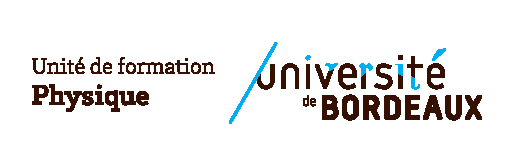
\includegraphics[height=2cm]{Logo_UF_Physique_cmjn.eps} 
			\end{flushleft}
		\end{minipage}
		\hfill
		\begin{minipage}{0.48\textwidth}
			\begin{flushright}
				
\includegraphics[height=2cm]{logo.png}
			\end{flushright}
		\end{minipage}
		
		\vspace{1.5cm} 
		\centering 
		
		{\large \MakeUppercase{Laboratoire d'Astrophysique de Bordeaux}} \\
		\vspace{0.2cm}
		\hrule
		
		\vfill
		
		{\huge \bfseries Lien entre la cinématique des étoiles jeunes et la cinématique du gaz moléculaire dans le complexe moléculaire géant Cygnus-X} \\[0.6cm]
		
		{\Large \textit{Rapport de stage de Master 1 Physique fondamentale et applications Parcours Noyaux, Particules et Univers}} \\
		
		\vfill
		
		{\large Présenté par :} \\
		{\Large \textbf{Sulwen de la Croix}} \\
		
		\vfill \vfill 
		
		
		\begin{minipage}{0.48\textwidth}
			\begin{flushleft} \large
				\textbf{Tuteur de stage :} \\
				M. Sylvain Bontemps\\
				\small Laboratoire d'Astrophysique de Bordeaux - Groupe FEMIS \\
				\small Directeur de recherche au CNRS
			\end{flushleft}
		\end{minipage}
		\hfill
		\begin{minipage}{0.48\textwidth}
			\begin{flushright} \large
				\textbf{Professeur référent :} \\
				Mme Marie-Hélène Grondin \\
				\small Laboratoire de Physique des 2 infinis (LP2i) Bordeaux
			\end{flushright}
		\end{minipage}
		
		\vfill
		
		
		\hrule
		\vspace{0.3cm}
		{\large Mai-Juin 2026} 
		
	\end{titlepage}
	
	\section*{Remerciements}
	%\addcontentsline{toc}{section}{Remerciements}
	Je tiens à exprimer ma profonde gratitude à M. Sylvain Bontemps pour son accueil au sein du Laboratoire d’Astrophysique de Bordeaux. Son accompagnement, à la fois pédagogique et ouvert, m’a permis de progresser tout en explorant librement les aspects du sujet qui m’intéressaient.
	
	Mes remerciements s’adressent également à Mmes Marie-Hélène Grondin et Yasmine Bercy ainsi qu'à M. Jean-Christophe Delagnes pour leur soutien, tant lors de la recherche de stage qu’au cours de son déroulement.
	
	Je suis reconnaissant envers MM. Yassin Khalil et Benoit Famaey (Université de Strasbourg) pour leur collaboration enrichissante et bienveillante, qui a grandement contribué à approfondir cette analyse cinématique.
	
	Enfin je souhaite remercier mes co-stagiaires Elise Peris, Quentin Sabucco et Corentin Canu.
	
	\tableofcontents
	\newpage
	\setcounter{page}{1}
	\section{Introduction}
	La région du Cygne (Cygnus X) constitue l'un des complexes moléculaires géants les plus massifs et actifs de notre galaxie, ce qui en fait un objet d'étude pertinent pour analyser les processus de formation stellaire. Les observations montrent qu'elle est composée de nuages denses où se forment actuellement des étoiles massives. L’un des mécanismes proposés pour expliquer la genèse de ces amas repose sur la collision de nuages moléculaires. Les travaux de N. Schneider et al. \cite{schneider2023} indiquent que l'interaction de nuages proches, animés de vitesses différentielles importantes, engendre une concentration du gaz propice à la formation d’étoiles massives. Pour tester cette hypothèse à l'échelle du complexe, une caractérisation précise de la cinématique spatiale des structures existantes est requise.
	
	À ce jour, la dynamique de Cygnus X a été documentée par des études indépendantes. Rygl et al. \cite{rygl2012} ont déterminé les distances et mouvements propres de plusieurs nuages à l'aide de masers. Parallèlement, Quintana et al. \cite{quintana2021} ont caractérisé la cinématique de plusieurs groupes d’étoiles massives OB au sein de cette même région. Si le modèle des collisions s'applique à Cygnus X, ces jeunes amas stellaires devraient conserver une trace cinématique des vitesses différentielles importantes de leurs nuages parents. Toutefois, aucune étude n'a encore croisé ces deux ensembles de données. Les référentiels de travail et les modèles de potentiel galactique utilisés dans ces publications diffèrent, ce qui empêche une comparaison analytique directe. Il est donc nécessaire de réévaluer ces mesures en adoptant un cadre d'analyse commun.
	
	Ce stage a pour objectif d'harmoniser ces jeux de données. Les positions et les vitesses observationnelles étant initialement projetées sur le plan du ciel, l'évaluation des distances relatives est limitée par des effets de perspective. La première étape consistera à exprimer les coordonnées et les vecteurs vitesse des nuages et des amas OB dans un repère galactocentrique cartésien unique. Cette conversion en trois dimensions permettra de s'affranchir des biais de projection et d'évaluer les relations spatiales actuelles de manière objective.
	
	Dans un second temps, l'exploitation de ces paramètres unifiés permettra d'extrapoler les trajectoires des amas vers le passé (traceback). L'objectif de cette méthode cinématique est d'identifier les époques de convergence maximale afin de reconstituer la configuration spatiale de Cygnus X lors des événements anciens de formation stellaire. Les données obtenues serviront à construire un scénario décrivant la chronologie dynamique de la région sur 10 à 15 Myr. Enfin, la mise en relation de cette chronologie avec la position de l'onde spirale permettra de confirmer que le Bras Local joue un rôle clé dans la dynamique et les interactions des nuages moléculaires.
	
	\setcounter{page}{1}
	\section{Cinématique des nuages moléculaires et des groupes d'étoiles massives}
	
	\subsection{Notions cinématiques}
	L'analyse de la dynamique des structures de la région du Cygne repose sur plusieurs concepts fondamentaux de la cinématique galactique. Les composantes de la vitesse particulière d'un objet par rapport au référentiel local sont définies par les variables cartésiennes $U$, $V$ et $W$ :
	\begin{itemize}
		\item $U$ : la composante radiale galactocentrique, projetée le long du rayon reliant l'objet au centre de la Galaxie. Selon la convention adoptée, une valeur positive de $U$ indique un mouvement dirigé vers le centre galactique.
		\item $V$ : la composante tangentielle, orientée dans le sens de la rotation galactique. Une valeur positive de $V$ signifie que l'objet possède une vitesse de rotation supérieure à celle du repère de référence.
		\item $W$ : la composante perpendiculaire au plan galactique. Une valeur positive indique un déplacement vers le pôle Nord galactique.
	\end{itemize}
	
	Le Référentiel Local au Repos, ou \textit{Local Standard of Rest} (LSR), est défini comme un repère idéal situé à la distance du Soleil du centre galactique ($R_0$) et corrigé de la vitesse du Soleil en suivant la convention IAU.
	
	Le référentiel galactocentrique cartésien a pour origine le centre galactique, l'axe $\vec{x}$ est la droite formée par le point étudié (par exemple le Soleil) et le centre galactique, avec pour convention une valeur positive lorsque l'on se rapproche du centre galactique. L'axe $\vec{y}$ est la droite orthogonale à l'axe des abscisses dans le plan galactique, les valeurs sont positives dans le sens de la rotation galactique. L'axe $\vec{z}$ pointe vers le pôle nord galactique, il est donc orthogonal au plan galactique. Une représentation du référentiel cartésien galactocentrique est disponible en figure  \ref{fig:galactocentric_cartesian}.
	
	\begin{figure}[H]
		\centering
		\begin{minipage}{0.9\textwidth}
			\centering
			\includegraphics[height=5cm]{galactocentric_cartesian.png}
			\caption{Référentiel galactocentrique cartésien avec le Soleil comme point d'étude}
			\label{fig:galactocentric_cartesian}
		\end{minipage}
	\end{figure}
	
	
	Enfin, les mouvements propres correspondent au déplacement angulaire des objets projeté sur le plan du ciel. Ils expriment la dérive de la position apparente au cours du temps et sont mesurés en millisecondes d'arc par an ($\mathrm{mas}\cdot\mathrm{an}^{-1}$).
	
	\subsection{Paramètres fondamentaux du modèle galactique}
	Les mouvements observés depuis la Terre dépendent directement de la position et de la vitesse du Soleil au sein de la Galaxie. Le Soleil est situé à une distance $R_0$ du centre galactique, présente un écart vertical $Z_0$ par rapport au plan moyen du disque, et possède des composantes de vitesse particulière ($U_{\odot}$, $V_{\odot}$, $W_{\odot}$) par rapport au LSR. Ces constantes de référence varient sensiblement selon les modèles cinématiques adoptés dans la littérature.
	
	Les mouvements propres et les vitesses particulières $U, V, W$ des nuages moléculaires de Cygnus X ont été initialement publiés par Rygl et al. \cite{rygl2012} en adoptant les paramètres de Schönrich et al. \cite{schonrich2010}. Afin d'intégrer les contraintes observationnelles les plus récentes et de réduire les incertitudes de mon modèle, j'utilise les paramètres révisés issus des mesures de la Gravity Collaboration \cite{gravity2022} et de Bobylev et al. \cite{bobylev2026} basées sur Gaia DR3. La comparaison de ces deux jeux de paramètres est synthétisée dans le Tableau \ref{tab:comparatif_parametres}.
	
	\begin{table}[H]
		\centering
		\small
		\vspace{0.2cm}
		\begin{tabular}{l c c}
			\hline
			\textbf{Paramètre} & \textbf{Valeurs historiques} & \textbf{Valeurs révisées} \\
			& (Schönrich et al. \cite{schonrich2010}) & (Gravity Col. \cite{gravity2022} ; Bobylev \cite{bobylev2026}) \\
			\hline
			$R_0$ ($\mathrm{kpc}$) & $8.3$ & $8.277 \pm 0.041$ \\
			$\Theta_0$ ($\mathrm{km\cdot s^{-1}}$) & $236$ & $234.8 \pm 3.0$ \\
			$U_{\odot}$ ($\mathrm{km\cdot s^{-1}}$) & $11.10 \pm 0.71$ & $9.83 \pm 0.42$ \\
			$V_{\odot}$ ($\mathrm{km\cdot s^{-1}}$) & $12.24 \pm 0.47$ & $13.33 \pm 0.50$ \\
			$W_{\odot}$ ($\mathrm{km\cdot s^{-1}}$) & $7.25 \pm 0.35$ & $7.89 \pm 0.41$ \\
			\hline
		\end{tabular}
		\caption{Comparaison des paramètres du LSR et des composantes de vitesses particulières du soleil entre le modèle de Schönrich et al. et le modèle de Bobylev et al. utilisé dans cette étude.}
		\label{tab:comparatif_parametres}
	\end{table}
	
	Ces constantes mises à jour me servent de base pour l'unification des différents jeux de données dans le référentiel galactocentrique commun.
	
	\subsection{Détermination des positions et des vitesses dans le référentiel galactocentrique}
	
	L'étude de Quintana et al. \cite{quintana2021} fournit les mouvements propres ainsi que les distances héliocentriques des groupes d'étoiles OB de la région du Cygne. À partir de ces données astrométriques, je détermine la position spatiale absolue de ces objets dans le référentiel galactocentrique cartésien. 
	
	Dans un premier temps, je convertis les mouvements propres en vitesses particulières observées ($U_{obs}, V_{obs}, W_{obs}$) à l'aide de la bibliothèque Python \textit{astropy}. Je corrige ensuite ces vitesses du mouvement propre du Soleil afin de les exprimer dans le référentiel du \textit{Local Standard of Rest} (LSR) :
	\begin{equation}
		U_{lsr} = U_{obs} + U_{\odot} \quad ; \quad V_{lsr} = V_{obs} + V_{\odot} \quad ; \quad W_{lsr} = W_{obs} + W_{\odot}
	\end{equation}
	
	Les publications de référence fournissent les coordonnées spatiales en longitude ($l$) et latitude ($b$) galactiques, ainsi que la distance héliocentrique ($D$). J'effectue la transformation vers le référentiel galactocentrique cartésien ($X, Y, Z$) selon la géométrie illustrée par les Figures \ref{fig:geometry_plane} et \ref{fig:geometry_Z} :
	\begin{equation}
		X = -R_0 + D \cos(l) \cos(b) \quad ; \quad Y = D \sin(l) \cos(b) \quad ; \quad Z = D \sin(b)
	\end{equation}
	L'angle d'azimut galactocentrique $\beta$ est défini par $\beta = \arctan\left(\frac{Y}{-X}\right)$.
	
	\begin{figure}[H]
		\centering
		\begin{minipage}{0.45\textwidth}
			\centering
			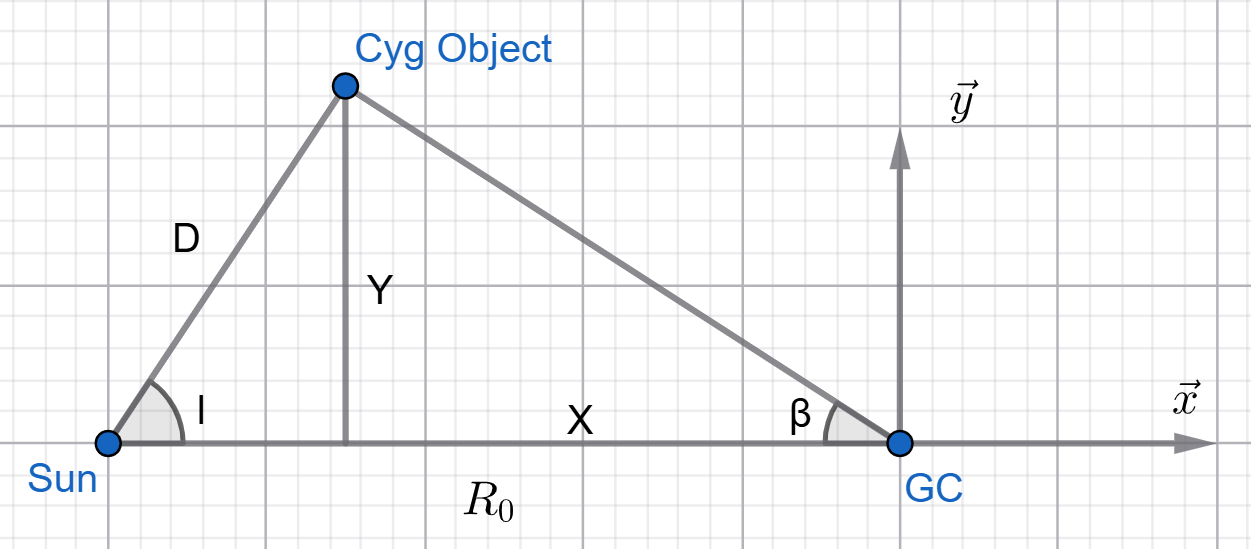
\includegraphics[height=2.5cm]{Cygnus_geometry_plane.png}
			\caption{Géométrie de projection dans le plan galactique ($X, Y$).}
			\label{fig:geometry_plane}
		\end{minipage}
		\hfill
		\begin{minipage}{0.45\textwidth}
			\centering
			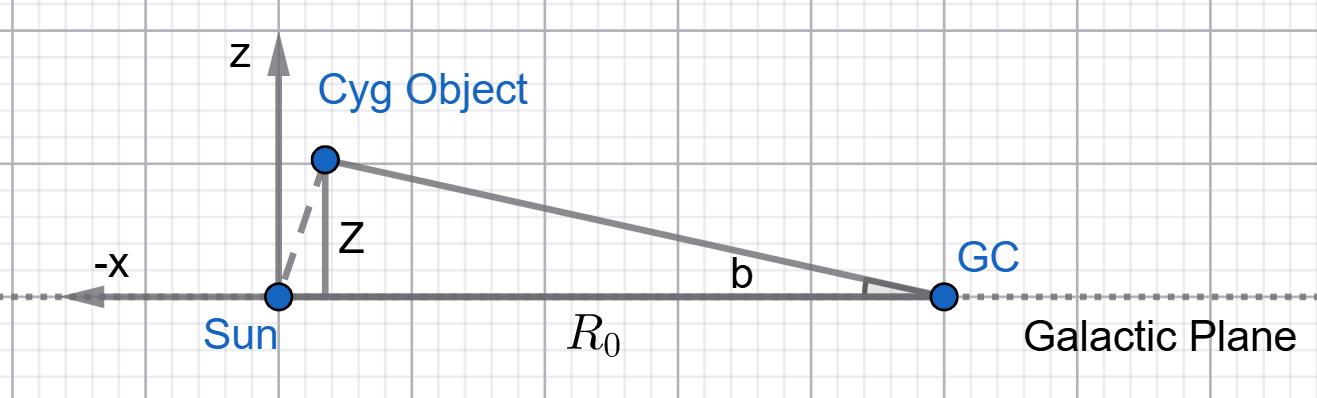
\includegraphics[height=2.5cm]{Cygnus_geometry_vertical.png}
			\caption{Géométrie de projection selon l'axe vertical ($Z$).}
			\label{fig:geometry_Z}
		\end{minipage}
	\end{figure}
	
	J'ajoute ensuite la vitesse de rotation circulaire moyenne de la Galaxie au niveau du Soleil ($\Theta_0$) pour obtenir la composante de vitesse galactocentrique absolue. Ce terme n'affecte que la composante tangentielle :
	\begin{equation}
		U_{lsr,abs} = U_{lsr} \quad ; \quad V_{lsr,abs} = V_{lsr} + \Theta_0 \quad ; \quad W_{lsr,abs} = W_{lsr}
	\end{equation}
	
	Enfin, pour exprimer ces vitesses dans le repère local de l'objet, j'effectue une rotation des axes d'un angle $\beta$ (Figure \ref{fig:geometry_lsr_to_peculiar}). Je soustrais également la vitesse circulaire locale $\Theta_0$ pour isoler la composante de vitesse galactocentrique particulière, notée $V_{pec}$ :
	\begin{figure}[H]
		\centering
		\begin{minipage}{0.55\textwidth}
			\begin{align}
				U_{pec} &= U_{lsr,abs}\cos(\beta) - V_{lsr,abs}\sin(\beta) \\
				V_{pec} &= U_{lsr,abs}\sin(\beta) + V_{lsr,abs}\cos(\beta) - \Theta_0 \\
				W_{pec} &= W_{lsr,abs}
			\end{align}
		\end{minipage}
		\hfill
		\begin{minipage}{0.40\textwidth}
			\centering
			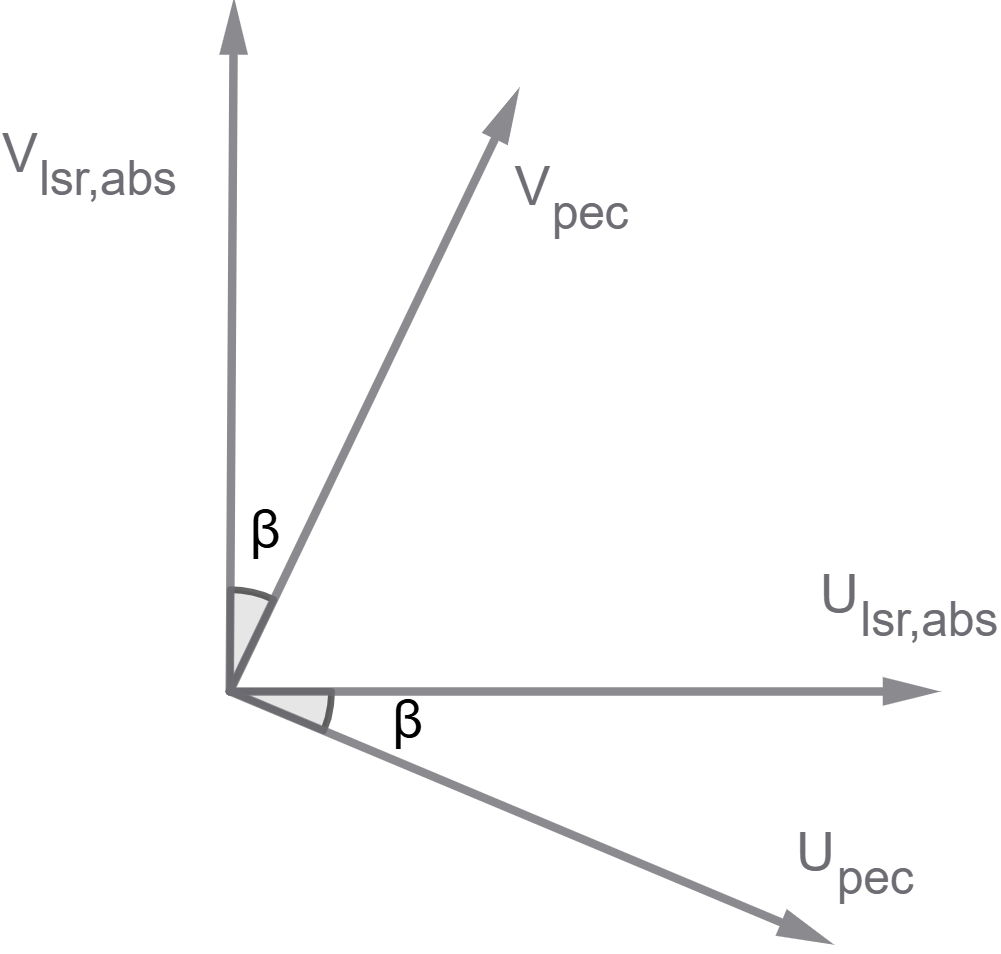
\includegraphics[width=\textwidth, height=4cm, keepaspectratio]{Transform_Vlsr_Vpec.png}
			\caption{Représentation géométrique de la rotation des axes cinématiques vers le référentiel galactocentrique.}
			\label{fig:geometry_lsr_to_peculiar}
		\end{minipage}
	\end{figure}
	
	Ces composantes ($U_{pec}, V_{pec}, W_{pec}$) sont celles que j'utiliserai dans la suite de ce rapport pour comparer les objets entre eux et établir les trajectoires de collision. 
	
	Cependant, pour faciliter la comparaison avec d'autres études et visualiser ces mouvements en 2D, je projette également ces vecteurs sur le plan du ciel. J'obtiens ainsi les vitesses propres en longitude ($v_l$) et en latitude ($v_b$):
	\begin{align}
		v_l &= -U_{pec}\sin(l) + V_{pec}\cos(l) \\
		v_b &= -U_{pec}\cos(l)\sin(b) - V_{pec}\sin(l)\sin(b) + W_{pec}\cos(b)
	\end{align}
	J'obtiens ainsi la norme du vecteur vitesse projeté sur le plan du ciel : $v_{lb} = \sqrt{v_l^2 + v_b^2}$.
	
	L'ensemble des résultats cinématiques appliqués aux nuages moléculaires et aux groupes d'étoiles OB de Cygnus X est compilé dans le Tableau \ref{tab:donnees_cinematiques}. Les distances d'entrée proviennent des travaux de Rygl et al. \cite{rygl2012} pour les nuages et de Quintana et al. \cite{quintana2021} pour les amas. 
	
	Les données astrométriques brutes utilisées pour initialiser ce modèle sont répertoriées dans le Tableau \ref{tab:annexe_donnees_entree} (Annexe \ref{annexe:donnees_complémentaires}). Les résultats intermédiaires qui ne sont pas directement utiles à l'argumentaire sont disponibles en annexe: les coordonnées spatiales héliocentriques (Tableau \ref{tab:annexe_positions}), les changements de référentiels de vitesse (Tableau \ref{tab:annexe_vitesses_intermediaires}) et enfin les propriétés internes des amas stellaires (Tableau \ref{tab:annexe_masses_gradients}).
	
	Pour les transformations linéaires, je calcule les incertitudes via la formule de propagation des erreurs au premier ordre (Taylor \cite{taylor1997}). Pour les fonctions non linéaires, j'effectue un échantillonnage par méthode de Monte-Carlo comprenant $10\,000$ tirages. Les calculs d'incertitudes détaillés sont documentés en Annexe \ref{annexe:methode_incertitudes}.

	
	\begin{table}[H]
		\centering
		\vspace{0.2cm}
		\resizebox*{\textwidth}{!}{
		\begin{tabular}{l c c c c c c c}
			\hline
			\textbf{Objet} & \textbf{Distance} & $\mathbf{U_{pec}}$ & $\mathbf{V_{pec}}$ & $\mathbf{W_{pec}}$ & $\mathbf{v_l}$ & $\mathbf{v_b}$ & $\mathbf{v_{lb}}$ \\
			& ($\mathrm{pc}$) & ($\mathrm{km/s}$) & ($\mathrm{km/s}$) & ($\mathrm{km/s}$) & ($\mathrm{km/s}$) & ($\mathrm{km/s}$) & ($\mathrm{km/s}$) \\
			\hline
			Group A & $1900 \pm 10$ & $14 \pm 2$ & $-12 \pm 3$ & $-5 \pm 2$ & $-17 \pm 2$ & $-4 \pm 2$ & $18 \pm 2$ \\
			Group B & $1730 \pm 10$ & $3 \pm 4$ & $-15 \pm 10$ & $2 \pm 2$ & $-6 \pm 4$ & $2 \pm 2$ & $6 \pm 4$ \\
			Group C & $1710 \pm 10$ & $11 \pm 2$ & $-16 \pm 3$ & $-2 \pm 1$ & $-15 \pm 2$ & $-2 \pm 1$ & $15 \pm 2$ \\
			Group D & $2000 \pm 10$ & $3 \pm 2$ & $-4 \pm 4$ & $-5 \pm 1$ & $-3 \pm 2$ & $-5 \pm 1$ & $6 \pm 2$ \\
			Group E & $1670 \pm 10$ & $-2 \pm 2$ & $-6 \pm 2$ & $0 \pm 2$ & $1 \pm 2$ & $0 \pm 2$ & $2 \pm 2$ \\
			Group F & $1990 \pm 10$ & $7 \pm 3$ & $-12 \pm 5$ & $-5 \pm 1$ & $-10 \pm 3$ & $-5 \pm 1$ & $11 \pm 3$ \\
			W75N & $1300 \pm 70$ & $-1 \pm 2$ & $-0.1 \pm 0.4$ & $1.8 \pm 0.3$ & $1 \pm 2$ & $1.9 \pm 0.3$ & $2.3 \pm 0.9$ \\
			DR21 & $1500 \pm 80$ & $-1 \pm 2$ & $-12.1 \pm 0.5$ & $7.3 \pm 0.2$ & $-1 \pm 2$ & $7.4 \pm 0.2$ & $7.5 \pm 0.3$ \\
			DR20 & $1460 \pm 90$ & $7 \pm 3$ & $-12.6 \pm 0.6$ & $5.8 \pm 0.2$ & $-9 \pm 2$ & $5.8 \pm 0.2$ & $10 \pm 2$ \\
			IRAS20290 & $1360 \pm 120$ & $1 \pm 3$ & $-12.0 \pm 0.7$ & $6.6 \pm 0.2$ & $-3 \pm 3$ & $6.8 \pm 0.2$ & $8 \pm 1$ \\
			\hline
		\end{tabular}
		}
		\caption{Paramètres cinématiques et distances héliocentriques des objets de Cygnus X.}
		\label{tab:donnees_cinematiques}
	\end{table}
	
	\subsection{Remarque sur les incertitudes et la crédibilité des résultats}
	Il est intéressant de comprendre quelles sont les incertitudes de mesures qui ont le plus d'impact sur les interprétations dynamiques à venir. La propagation des erreurs sur la vitesse du soleil et les distances aboutit à des incertitudes élevées sur les composantes de vitesses, par exemple, on trouve pour le groupe D une vitesse tangentielle de: $V_{pec} \ = \ -3.62 \ \pm \ 3.72 \ km/s$. Avec une telle incertitude, on pourrait penser qu’aucune interprétation valable ne peut être faite des résultats. Cependant, la majorité de cette incertitude est due à la marge d'erreur sur la vitesse tangentielle du soleil issue de Bobylev et al. \cite{bobylev2026} et cette vitesse tangentielle du soleil s'applique de manière identique à tous les objets étudiées. Or notre étude porte sur les mouvements relatifs des objets entre eux, ainsi, même si l’incertitude sur la valeur absolue est importante, elle s’annule lorsque l’on étudie le mouvement des groupes d’étoiles et des nuages de moléculaires les uns par rapport aux autres. De même, l’incertitude sur la vitesse de rotation de la galaxie au niveau du soleil ou de Cygnus-X n’intervient pas dans les mouvements relatifs des objets entre eux.
	
	Les sources d'incertitudes dominantes ayant un réel impact sur les interprétations sont les mesures des vitesses radiales des groupes d'étoiles OB issues de Quintana et al. \cite{quintana2022} et les mesures de distances et de mouvements propres des nuages moléculaires issues de Rygl et al. \cite{rygl2012}. Une meilleure précision de ces mesures astronomiques permettrait de réduire les incertitudes sur les vitesses particulières des objets du Cygne.
	
	Afin de s'assurer de la véracité des calculs de changements de référentiels effectués, j'ai calculé les vitesses particulières des nuages moléculaires en utilisant les paramètres de Schönrich et al. \cite{schonrich2010}. J'ai retrouvé exactement les mêmes valeurs que Rygl et al. \cite{rygl2012}. J'ai aussi mesuré la taille des flèches sur la Figure 12 de Rygl et al. \cite{rygl2012}, puis je les aies converties en km/s grâce à l'échelle du graphique (2.3 cm = 10 km/s). J'obtiens:
	
	\begin{itemize}
		\item W75N : $v_{cm} = 0.35 \pm 0.1 \, \mathrm{cm} \Leftrightarrow v_{UW} = 1.5 \pm 0.4 \, \mathrm{km/s}$
		\item DR21 : $v_{cm} = 1.6 \pm 0.1 \, \mathrm{cm} \Leftrightarrow v_{UW} = 6.7 \pm 0.4 \, \mathrm{km/s}$
		\item DR20 : $v_{cm} = 2.1 \pm 0.1 \, \mathrm{cm} \Leftrightarrow v_{UW} = 9.1 \pm 0.4 \, \mathrm{km/s}$
		\item IRAS 20290+4052 : $v_{cm} = 1.5 \pm 0.1 \, \mathrm{cm} \Leftrightarrow v_{UW} = 6.5 \pm 0.4 \, \mathrm{km/s}$
	\end{itemize}
	Je compare cela aux vitesses calculées pour les mêmes hypothèses (Schönrich et al. \cite{schonrich2010}):
	\begin{align*}
		U_{W75N, \text{calculée}} &= -0.53 \, \text{km/s}; \qquad W_{W75N, \text{calculée}} = 1.23 \, \text{km/s} \\
		v_{W75N, \text{calculée}} &= \sqrt{ U_{W75N, \text{calculée}}^2 + W_{W75N, \text{calculée}}^2 } = 1.3 \, \text{km/s} \\[0.5cm]
		U_{DR21, \text{calculée}} &= -0.03 \, \text{km/s}; \qquad W_{DR21, \text{calculée}} = 6.62 \, \text{km/s} \\
		v_{DR21, \text{calculée}} &= \sqrt{ U_{DR21, \text{calculée}}^2 + W_{DR21, \text{calculée}}^2 } = 6.7 \, \text{km/s} \\[0.5cm]
		U_{DR20, \text{calculée}} &= 7.5 \, \text{km/s}; \qquad\quad\; W_{DR20, \text{calculée}} = 5.11 \, \text{km/s} \\
		v_{DR20, \text{calculée}} &= \sqrt{ U_{DR20, \text{calculée}}^2 + W_{DR20, \text{calculée}}^2 } = 9.1 \, \text{km/s} \\[0.5cm]
		U_{IRAS20290, \text{calculée}} &= 1.89 \, \text{km/s}; \qquad W_{IRAS20290, \text{calculée}} = 5.96 \, \text{km/s} \\
		v_{IRAS20290, \text{calculée}} &= \sqrt{ U_{IRAS20290, \text{calculée}}^2 + W_{IRAS20290, \text{calculée}}^2 } = 6.3 \, \text{km/s}
	\end{align*}
	\begin{align*}
		\Delta v_{UW, W75N} &= |v_{UW, \text{mesurée}, W75N} - v_{UW, \text{calculée}, W75N}| = |1.5 - 1.3| = 0.2 \pm 0.6 \, \text{km/s} \\[0.2cm]
		\Delta v_{lb, DR21} &= |v_{lb, \text{mesurée}, DR21} - v_{lb, \text{calculée}, DR21}| = |6.7 - 6.7| = 0 \pm 0.6 \, \text{km/s} \\[0.2cm]
		\Delta v_{lb, DR20} &= |v_{lb, \text{mesurée}, DR20} - v_{lb, \text{calculée}, DR20}| = |9.1 - 9.1| = 0 \pm 0.6 \, \text{km/s} \\[0.2cm]
		\Delta v_{lb, IRAS20290} &= |v_{lb, \text{mesurée}, IRAS20290} - v_{lb, \text{calculée}, IRAS20290}| = |6.5 - 6.3| = 0.2 \pm 0.6 \, \text{km/s}
	\end{align*}
	Les résultats concordent dans la limite des incertitudes utilisées, on peut donc en conclure que la méthode de calcul des vitesses est cohérente avec l’article de Rygl et al. \cite{rygl2012}, et donc commencer à interpréter les résultats.
	
	\section{Visualisation des vitesses et des positions}
	\subsection{Projection en deux dimensions}
	J'utilise NASA Sky View pour récupérer une image de Cygnus-X provenant d'une observation du télescope WISE à 12 $\mu$m. A cette longueur d'onde, WISE montre les poussières chaudes à l'interface entre les nuages et le rayonnement UV des étoiles jeunes massives. Le fichier FITS extrait peut ensuite être chargé comme image d'arrière-plan via la bibliothèque \textit{astropy} de python. Le graphique représentant les positions et les vitesses $v_l$ et $v_b$ projetées sur l'image du Cygne est disponible en figure \ref{fig:cygnus_fits}.
	
	\begin{figure}[H]
		\centering
		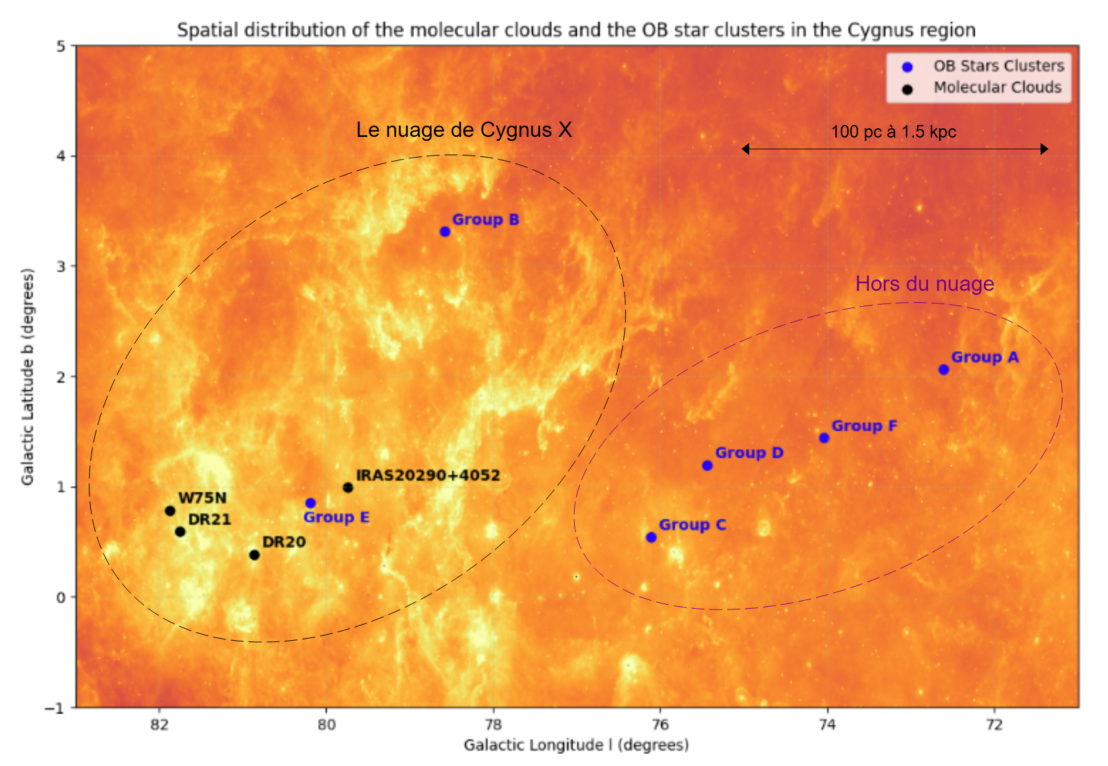
\includegraphics[height=8cm]{spatial_distribution_legended.png}
		\caption{Projection des positions et des vitesses des nuages moléculaires et des groupes d'étoiles massives sur une image WISE à 12 $\mu$m. L'abscisse est la longitude galactique et l'ordonnée la latitude galactique. Les nuages moléculaires sont en bleus et les groupes d'étoiles en vert et rouge. Les vitesses sont corrigées de la vitesse particulière du Soleil et de la vitesse de rotation moyenne de la galaxie $\Theta_0$}
		\label{fig:cygnus_fits}
	\end{figure}
	A cette longueur d'onde, les nuages moléculaires sont bien visibles mais les groupes d'étoiles ne le sont pas directement. Indirectement, on voit des bulles au niveau des groupes d'étoiles qui éjectent la matière environnante par de forts vents stellaires. Le groupe E semble très proche des nuages moléculaires, cependant cette vue ne tient pas compte des distances des objets sur la ligne de visée, donc de la profondeur sur le graphique, et le groupe E est en réalité environ 300 pc plus lointain que les nuages moléculaires. On peut aussi voir que le groupe B est sur une latitude galactique plus élevée que les autres objets. Les vitesses $v_l$ et $v_b$ permettent de visualiser les trajectoire des nuages et des groupes d'étoiles dans ce plan.

	La figure \ref{fig:cygnus_fits} nous permet de voir que les groupes A, B, C, D et F se dirigent tous vers le centre de la galaxie alors que le groupe E lui est presque immobile par rapport à la rotation moyenne de la galaxie. Pour les nuages, le groupe W75N suit lui aussi la vitesse de rotation moyenne alors que les nuages DR20, DR21 et IRAS20290+4052 sont entrainés vers le pôle nord galactique et plutôt vers le centre de la galaxie.
		
	Afin d'apprécier les distances des objets au soleil, je projette les vitesses $U_{pec}$ et $V_{pec}$ des objets sur le plan galactique en figure \ref{fig:bobylev_U_V_plane}. La vitesse $U_{pec}$ est positive selon l'axe des ordonnées et la vitesse $V_{pec}$ est positive selon l'axe des abscisses. Le vecteur résultant est la somme de ces deux vitesses. Je prends pour origine le nuage W75N pour se placer dans un référentiel local, car c'est ce nuage qui se déplace selon la courbe de rotation standard de la galaxie et qui se situe sur le plan galactique, de plus c'est au niveau des nuages actuels que se déroule la formation d'étoiles. Il est donc nécessaire d'effectuer une translation du repère galactocentrique en utilisant $X(W75N)$ et $Y(W75N)$, les coordonnées de W75N dans le référentiel galactocentrique. Je trace aussi les positions et les vitesses des objets du Cygne dans le plan (X,Z) en figure \ref{fig:X_Z_plane}, ce qui permet de voir la hauteur des objets au-dessus du plan galactique.
	
	\begin{figure}[H]
		\centering
		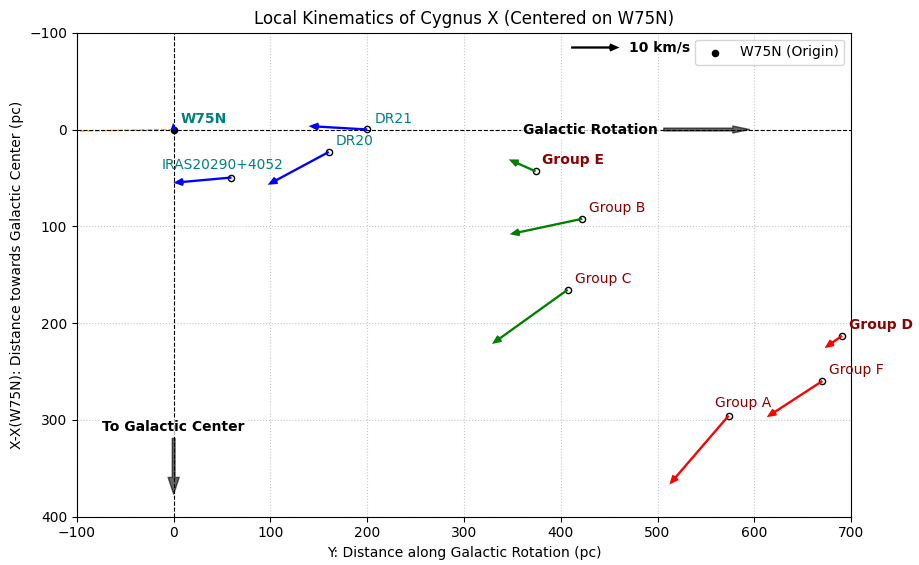
\includegraphics[height=8cm,keepaspectratio]{Galactic plane view Bobylev 2026 v2.png}
		\caption{Projection des vitesses $U_{pec}$ et $V_{pec}$ des nuages moléculaires et des groupes d'étoiles massives sur le plan galactique. L'abscisse est la distance selon la rotation de la galaxie et l'ordonnée est la distance vers le centre galactique. La ligne jaune indique la direction du Soleil. Les nuages moléculaires sont en bleu et les groupes d'étoiles en rouge et vert.}
		\label{fig:bobylev_U_V_plane}
	\end{figure}
	\begin{figure}[H]
		\centering
		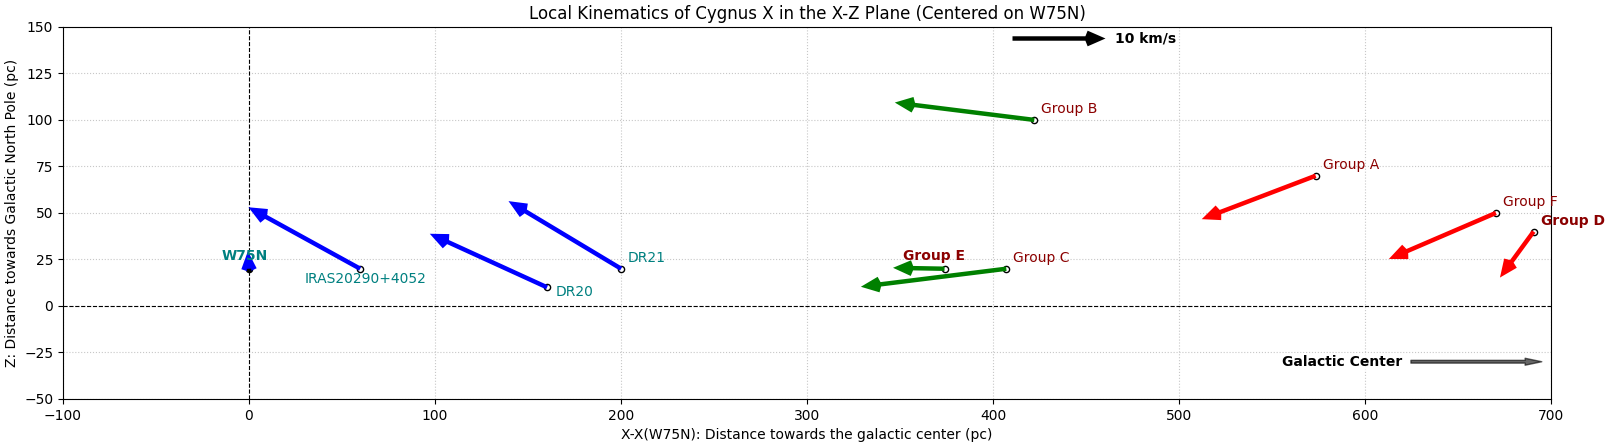
\includegraphics[height=4cm,keepaspectratio]{Kinematics_XZ_plane.png}
		\caption{Projection des vitesses $U_{pec}$ et $W_{pec}$ des nuages moléculaires et des groupes d'étoiles massives dans le plan (X,Z). L'abscisse est la distance vers le centre Galactique et l'ordonnée est la distance vers le pôle Nord Galactique. . Les nuages moléculaires sont en bleu et les groupes d'étoiles en rouge et vert.}
		\label{fig:X_Z_plane}
	\end{figure}
	
	En comparant avec la figure \ref{fig:cygnus_fits}, on se rend compte que les interprétations qui se basent uniquement sur la projection sur le plan du ciel et qui ne prennent pas en compte la distance sur la ligne de visée peuvent être erronées. En effet, même si la figure \ref{fig:cygnus_fits} nous fait penser que le groupe E fait partie du nuage, la figure \ref{fig:bobylev_U_V_plane} nous permet de distinguer plutôt trois super-amas d'objets distincts. Les deux super-groupes d'étoiles massives BEC et FAD, et le groupe des nuages moléculaires. Chacun de ces deux super-amas est espacé d'environ 200 parsecs dans la direction de la rotation de la galaxie.
	
	Pour ne pas se limiter à des projections en 2D, on peut aussi faire une visualisation en 3D et étudier la cinématique sous différents angles.
		
	\subsection{Projection en trois dimensions}
	Afin de calculer les positions et les vitesses des objets en 3D, j'utilise le même repère que pour la représentation en 2D. La visualisation 3D est difficilement appréciable sur un support 2D, le fichier est disponible à \href{https://github.com/KyuriTaima/CygnusDynamics/blob/8276b42224d7c76e1cba126970f6e30ef20acc10/Carte_Cygnus_3D_quiver.html }{cette adresse}. Quelques vues 3D sont aussi disponibles en annexe \ref{appendix:complementary_graphs}, figures \ref{fig:3D_view_1} et \ref{fig:3D_view_2}.

	La visualisation 3D permet de se rendre compte des vitesses différentielles entre les objets. Au niveau du complexe de nuages moléculaires, W75N est presque immobile par rapport à la rotation de la Galaxie alors que les autres nuages sont ralentis de $14$ à $15 \ \mathrm{km\cdot s^{-1}}$ par rapport à la rotation moyenne de la galaxie, de plus, ils montent vers le pôle nord galactique. Au niveau du super-amas BEC, le groupe B est plus haut que les deux autres amas, mais les vitesses des groupes B et C sont similaires tandis que le groupe E a une vitesse beaucoup plus faible, et dans une direction différente. Il est proche de la rotation galactique comme le nuage W75N.
	
	Connaissant les vitesses et les positions des objets, je suis en capacité de revenir dans le passé pour étudier la cinématique des objets du Cygne à différentes temporalités clés. L'extrapolation de ces trajectoires a pour but de reconstituer la séquence chronologique d'apparition des amas massifs, dans l'optique de mettre en évidence un motif dynamique commun guidant l'évolution de Cygnus X.
	
	\section{Traceback des objets du Cygne}
	\subsection{Traceback linéaire des amas d'étoiles OB}
	Je peux effectuer un traceback linéaire des amas à partir des positions et des vitesses calculées. Bien que ce type de traceback de premier ordre soit très imprécis pour les intervalles de temps trop anciens, car il ne tient pas compte de la rotation de la galaxie ni des variations des influences gravitationnelles, il donne une bonne estimation des positions relatives des amas à moins de 10 millions d'années. Effectuer un traceback des nuages moléculaires n'a pas vraiment de sens car ils commencent seulement actuellement leur formation d'étoiles. 
	
	Les traceback linéaires des super-groupes BEC et FAD sur le plan galactique sont tracés en annexe \ref{appendix:complementary_graphs}, en figure \ref{fig:linear_traceback_BEC_XY} et \ref{fig:linear_traceback_FAD_XY}. Le calcul effectué pour tracer la position à chaque instant $t$ est détaillé en annexe \ref{appendix:linear_traceback}.
	
	On constate que les deux super-amas semblent avoir été les plus compacts il y a environ 10 millions d'années. Mais cette représentation comporte un biais important, car il s'agit d'une projection sur le plan XY et que, par conséquent, la composante Z n'est pas prise en compte. Or, nous avons montré que le groupe B se trouve en réalité en hauteur sur le plan XZ ; il faut donc également tenir compte de cette composante Z. 	
	
	Afin d'approfondir cette analyse, je peux déterminer le moment où les amas étaient les plus proches les uns des autres en appliquant la méthode des moindres carrés à des intervalles de 100 000 ans, entre 0 et 20 millions d'années. Je calcule la moyenne des distances entre les amas pour chaque intervalle de temps et détermine la valeur la plus faible. La valeur ainsi obtenue est le TCA (Time of Closest Approach), son calcul est détaillé en annexe \ref{appendix:linear_traceback}. Les résultats obtenus sont présentés en figure \ref{fig:traceback_TCA}.
	
	Pour le super-amas BEC, j'obtiens un TCA de $-3.3 \pm 1.8 \ \mathrm{Myr}$ avec une distance relative minimale de $100 \pm 12.3 \ \mathrm{pc}$. Pour le groupe FAD, j'obtiens un TCA de $-6.6 \pm \ 3.3 \ \mathrm{Myr}$ avec une distance relative minimale de $73 \pm 20.1 \ \mathrm{pc}$. Ces valeurs concordent parfaitement avec celles de Quintana et al. \cite{quintana2022}, qui datent les associations B, C et E de 3 à 5 millions d'années et les associations F, A et D d'environ 10 millions d'années.
	
	\begin{figure}[H]
		\centering
		\begin{minipage}{0.49\textwidth}
			\centering
			
\includegraphics[height=4.5cm]{TCA_MCC_BCE.png}
		\end{minipage}
		\hfill
		\begin{minipage}{0.49\textwidth}
			\centering
			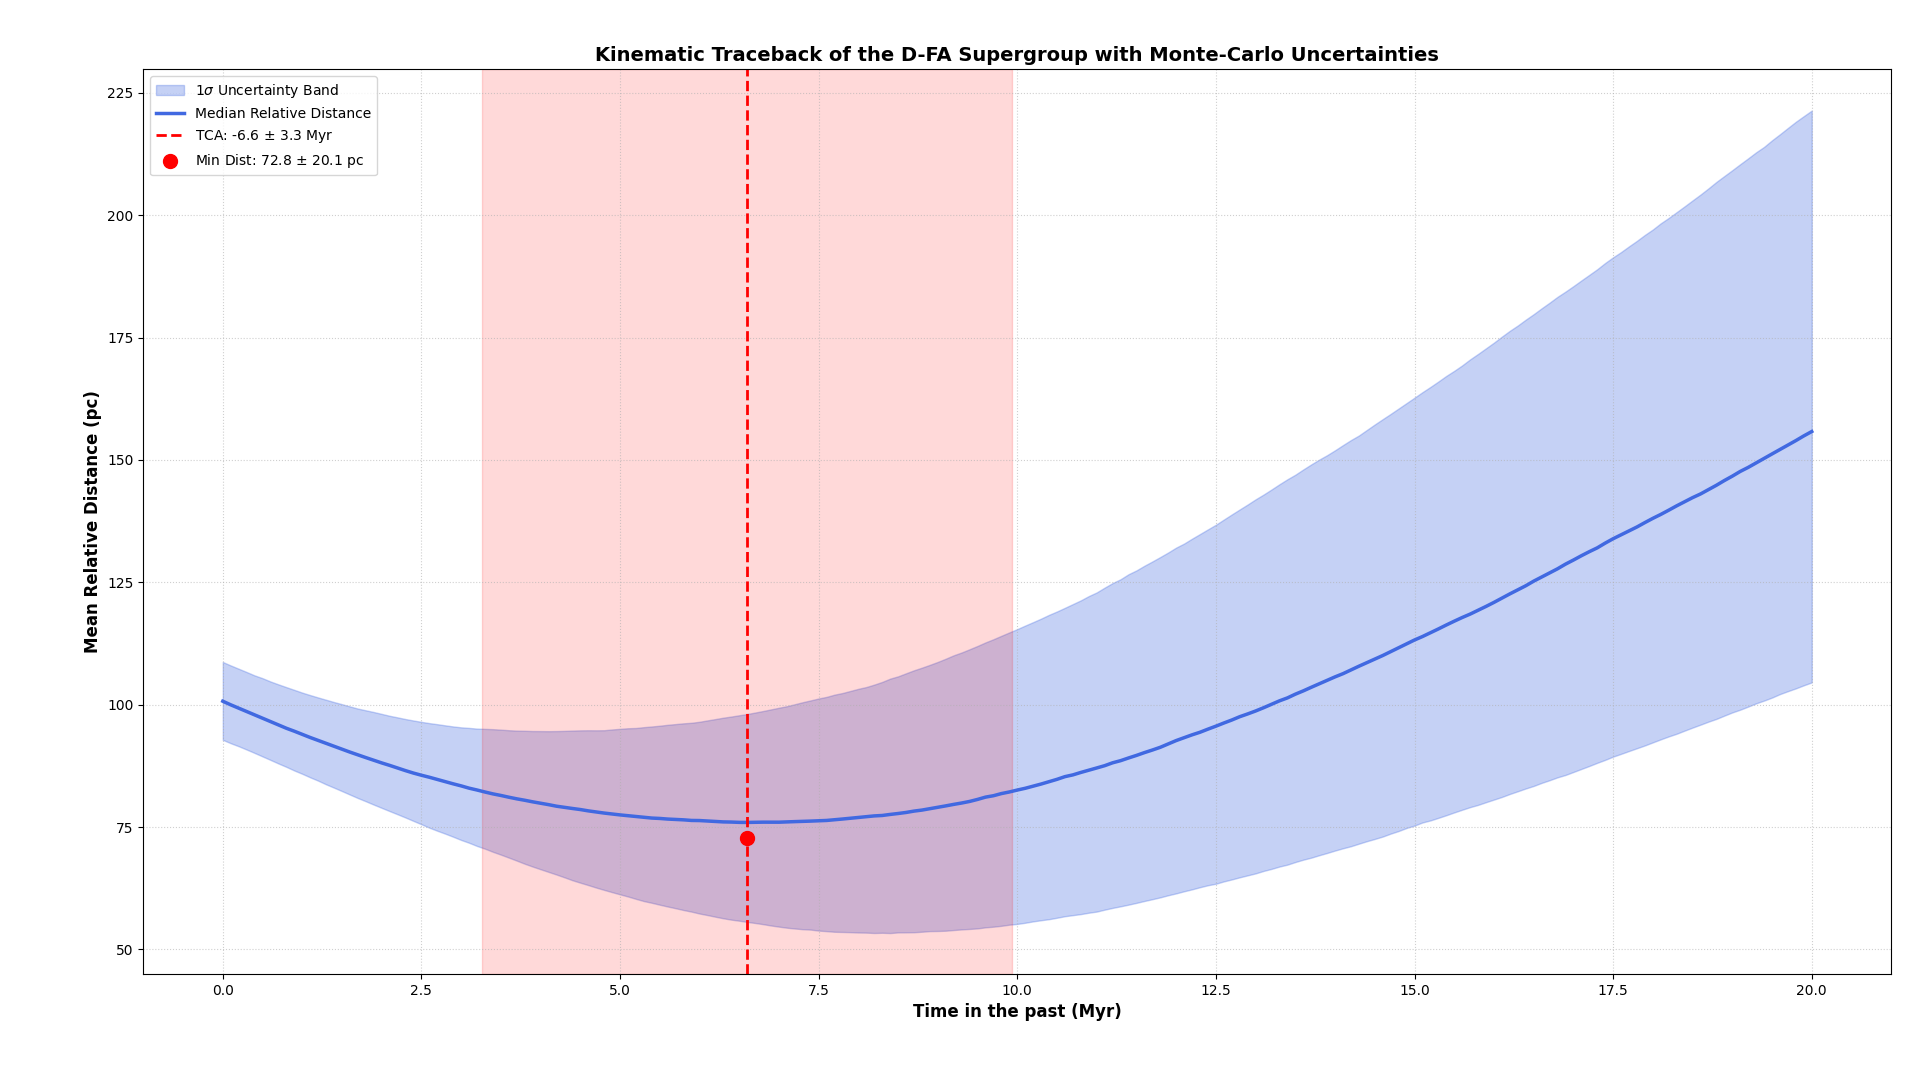
\includegraphics[height=4.5cm]{TCA_MCC_FAD.png}
		\end{minipage}
		\caption{Moyenne des distances entre les membres d'un même super-groupe en fonction du temps. Super-groupes: E-BC à gauche et D-FA à droite. Les incertitudes sont propagées par simulation de Monte-Carlo}
		\label{fig:traceback_TCA}
	\end{figure}
	
	Le groupe B se trouvant au-dessus du plan galactique, la force de rappel gravitationnelle qui le ramène vers le plan galactique n'est pas négligeable et je ne peux donc pas utiliser une approximation de vitesse linéaire, même pour quelques millions d'années en arrière. De plus, rien n'indique que le TCA devrait être le même entre E et C et entre E et B. Je détermine donc le TCA linéaire entre C et E, car ils se trouvent tous deux dans le plan galactique, et j'obtiens $-4.0 \pm 1.5 \ \mathrm{Myr}$ avec une distance relative minimale de $94 \ \pm 17.0 \mathrm{pc}$.
	
	Afin de comprendre la dynamique globale de la région du Cygne, je représente les positions des objets du Cygne aux deux instants clés: $-3.3 \ \mathrm{Myr}$ et $-6.6 \ \mathrm{Myr}$ sur la figure \ref{fig:traceback_mosaique}. Je représente aussi la disposition des objets du Cygne à $-10 \ \mathrm{Myr}$ et $-15 \ \mathrm{Myr}$ en annexe \ref{appendix:complementary_graphs}, figure \ref{fig:traceback_complémentaires}.
	
	La projection sur le plan galactique devrait être assez précise, car elle n'est pas influencée par la force de rappel du plan galactique, en revanche, la composante Z perd rapidement de sa précision, car les objets oscillent autour du plan galactique et devraient être ramenés vers le bas lorsqu'ils s'éloignent trop du plan galactique. Ainsi, bien qu'une vue en 3D soit intéressante, la projection sur le plan X,Y peut permettre de meilleures interprétations. Les vues 3D de ces instants clés sont disponibles en Annexe \ref{appendix:complementary_graphs}, figure \ref{fig:traceback_complémentaires_3D}.
	
	Sur la figure \ref{fig:traceback_mosaique}, on peut voir que le groupe E s'éloigne des groupes B et C à partir de $3.3 \ \mathrm{Myr}$ et que les groupes B et C sont très proches à $6.6 \ \mathrm{Myr}$ puis s'éloignent si on remonte plus loin dans le temps. Les groupes F,A et D se rapprochent jusqu'à $10 \ \mathrm{Myr}$ puis s'éloignent les uns des autres, jusqu'à ce que le groupe A se rapproche du groupe B vers $15 \ \mathrm{Myr}$. Les nuages moléculaires s'éloignent les uns des autres si on remonte dans le passé, ils sont donc actuellement plus proche les uns des autres qu'ils ne l'ont jamais été par le passé.
	Cette visualisation est très intéressante pour établir un scénario complet de formation de groupes d'étoiles massives, mais l'utilisation de vitesses linéaires a des limites si on revient à plus de 10 millions d'années dans le passé. Afin d'établir un état des lieux plus juste, on peut modéliser un potentiel gravitationnel local au niveau de la région du Cygne.
	
	
	\begin{figure}[H]
		\centering
		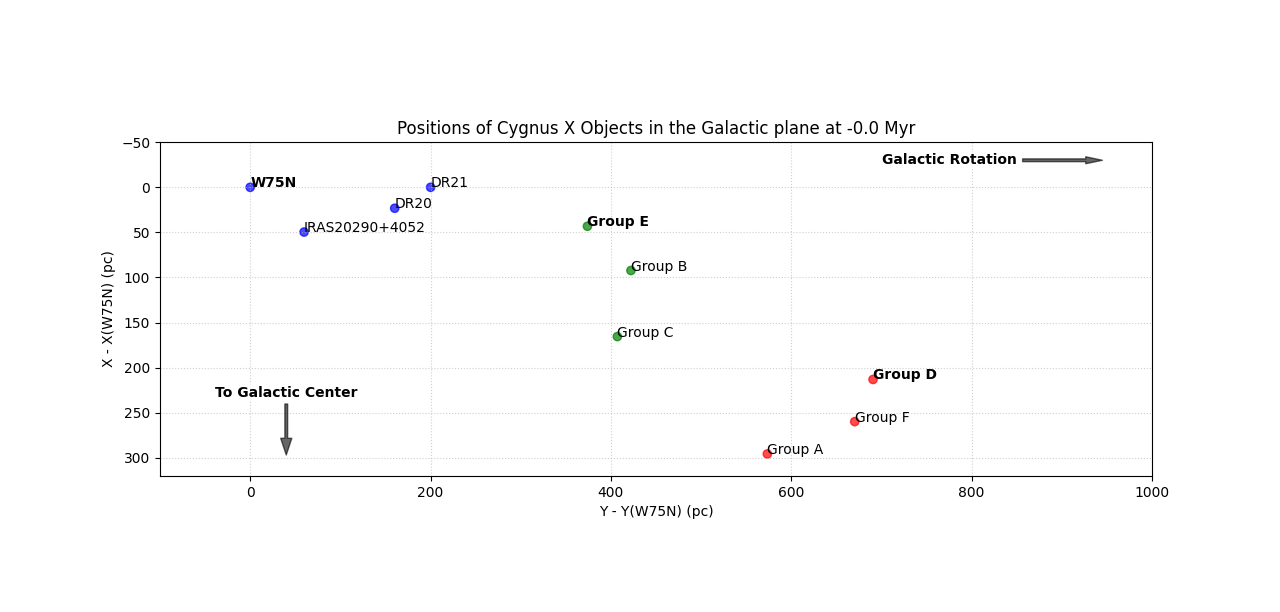
\includegraphics[width=0.8\textwidth, height=8cm, keepaspectratio]{traceback_gal_plane_0.png}
		
		\vspace{0.4cm}
		
		\centering
		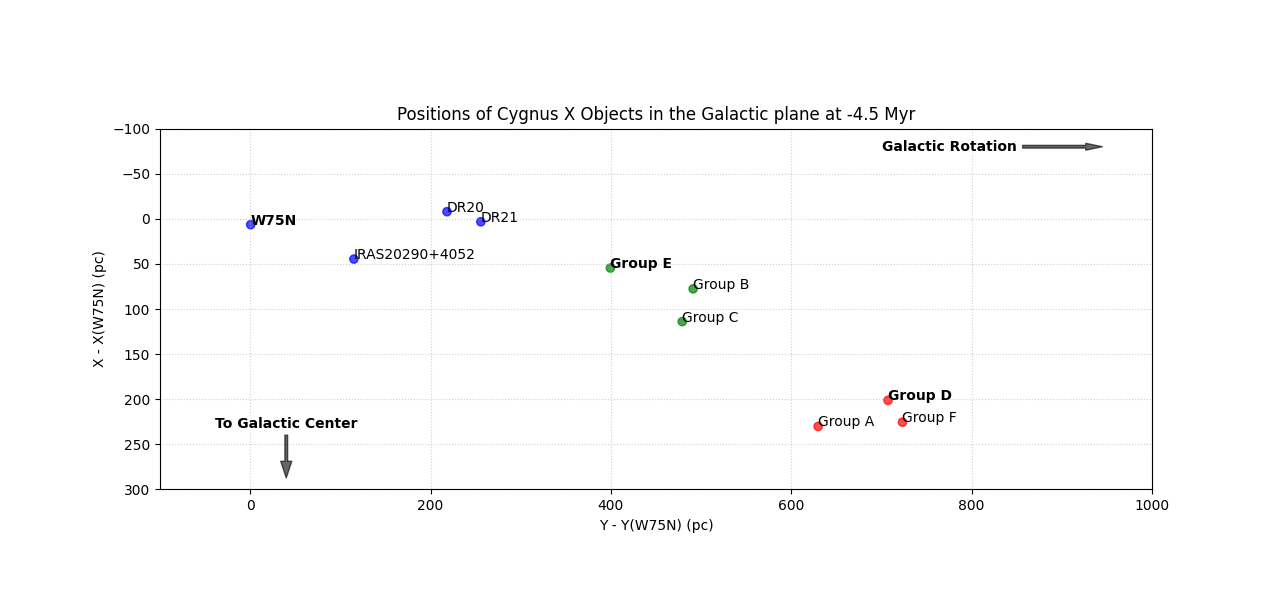
\includegraphics[width=0.8\textwidth, height=8cm, keepaspectratio]{traceback_gal_plane_4,5.png}
		
		\vspace{0.4cm}
		
		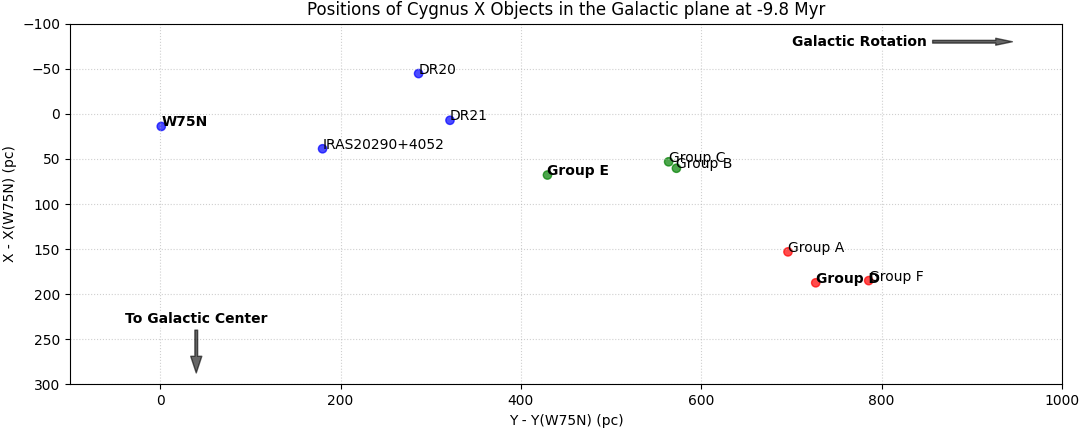
\includegraphics[width=0.8\textwidth, height=8cm, keepaspectratio]{traceback_gal_plane_9,8.png} 
		\caption{Traceback linéaire sur le plan galactique des objets du Cygne à  $0$, $-3.3$ et $-6.6 \ \mathrm{Myr}$. L'origine est le centre galactique, l'objet de référence est la position du nuage W75N actuellement. L'axe des abscisses est $Y$. L'axe des ordonnées est $X-X(W75N)$. Les nuages sont en bleu, les groupes d'étoiles OB en rouge et vert.}
		\label{fig:traceback_mosaique}
	\end{figure}
		

	\subsection{Traceback avec un potentiel gravitationnel local}
	Le potentiel gravitationnel local de la galaxie au niveau de la région du Cygne est complexe à modéliser, il nécessite des modèles de potentiels gravitationnels classiques avec plusieurs potentiels sphériques et disquaires, mais il nécessite aussi de prendre en compte l'influence gravitationnelle de la barre centrale galactique et des bras spiraux. En effet, dans le profil de densité de matière de la galaxie, on reconnait des motifs de sur-densité correspondant aux bras spiraux, ceux-ci sont difficiles à reproduire. Cependant, cette modélisation a récemment été réalisée par Yassin Khalil de l'université de Strasbourg, en utilisant la contrainte des dernières données de Gaia, avec une capacité à bien reproduire les motifs de sur-densité . Nous lui avons donc demandé d'effectuer un traceback des nuages et des amas d'étoiles massives à partir des positions et des vitesses calculées précédemment.
	
	Avec cette modélisation plus réaliste, nous obtenons un TCA de $-2.9^{+1.9}_{-2.7} \ \mathrm{Myr}$ pour le super-amas BCE et un TCA de $-6.9^{+3.0}_{-5.4} \ \mathrm{Myr}$. L'évolution de la distance entre les amas d'un même super-groupe en fonction du temps est disponibles en annexe \ref{appendix:complementary_graphs}, figure \ref{fig:TCA_nonaxi}. Ces résultats évoquent des évènements de formation similaires aux tracebacks linéaires.
	
	On peut comparer les TCA obtenus avec les âges stellaires estimés des groupes d'étoiles OB de la région du Cygne. La classification de Quintana et al. \cite{quintana2021} est récente et encore peu utilisée, il faut donc utiliser l'ancienne classification pour récupérer des âges stellaires dans diverses publications. Cependant il n'y a pas une parfaite correspondance entre les groupes des anciennes et nouvelles classifications, donc les âges stellaires de tous les groupes ne peuvent pas être identifiés dans la littérature. Le groupe E (Cygnus OB2) est le seul amas qui soit bien documenté, Berlanas et al. \cite{berlanas2020} datent les étoiles de 3 à 5 millions d'années, ce qui est cohérent avec le TCA obtenu. Comeron et al. \cite{comeron2020} déterminent que le début de la formation d'étoiles massives au sein de Cygnus OB1 (Groupes F,C et D) aurait commencé vers $15 \ \mathrm{Myr}$, ce qui est cohérent avec les TCA calculés pour le super-groupe FAD.
	
	\section{Scénario de formation des groupes d'étoiles massives au sein de la région du Cygne}
	\subsection{Processus de collision de nuages moléculaires}
	Avant de comprendre la dynamique globale de la région du Cygne, il est important de comprendre comment la collision de nuages moléculaires pourrait entrainer une formation de groupes d'étoiles massives. Les nuages moléculaires possèdent des formes variées et un gradient de densité associé. On peut distinguer la partie visible en infrarouge (et en raie moléculaire comme le CO) des nuages qui possèdent une densité de $10^5 \mathrm{cm^{-3}}$, et le halo de matière qui entoure le nuage avec une densité estimée de $50 \ \mathrm{cm^{-3}}$ à $200 \ \mathrm{cm^{-3}}$. La collision de deux nuages moléculaires n'a pas lieu entre les deux cœurs denses, mais correspond plutôt à la traversée du halo du premier nuage par le cœur dense du second nuage. Ces nuages moléculaires possèdent une structure filamentaire accompagnée d'un champ magnétique qui s'étend à $10 \ \mathrm{pc}$ au delà du filament. Lorsque le filament dense traverse le milieu peu dense du halo, le champ magnétique agit comme un râteau et accrète la matière vers le centre du filament et freine le filament qui peut aussi collecter la matière de son nuage. Cela permet donc d'augmenter la densité du cœur dense, et donc ultimement de former des étoiles plus massives.
	
	A partir de ce processus, on peut estimer la distance $l$ que doit parcourir le filament pour doubler sa masse initiale. On considère que le filament est un cylindre avec un rayon de $R_{fil} = 0.15 \ \mathrm{pc}$ et une densité $n_{fil} = 10^5 \ \mathrm{cm^{-3}}$ qui traverse un milieu avec une densité de $n_{halo} = 50 \ \mathrm{cm^{-3}}$. Le champ magnétique du filament a une longueur estimée à $d_B = 10 \ \mathrm{pc}$.
	On souhaite accréter autant de particules que le nombre de particules initiales: $$\pi R_{fil}^2 \times L_{fil} \times n_{fil} = 2R_B \times L_{fil} \times l \times n_{halo} \Leftrightarrow l \ = \ \frac{\pi}{2} \frac{R_{fil}^2}{R_B} \times \frac{n_{fil}}{n_{halo}} \ = \textbf{14.1 \ pc} $$.
	
	\begin{figure}[H]
		\centering
		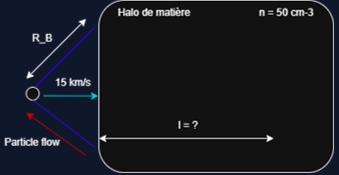
\includegraphics[height=5cm]{Filament_géométrie.png}
		\caption{Schéma représentant la traversée d'un filament à gauche à travers le halo d'un nuage à droite}
		\label{fig:collision nuages}
	\end{figure}
	
	Avec une vitesse de $15 \ \mathrm{pc} \cdot \mathrm{Myr^{-1}} \Leftrightarrow 15 \ \mathrm{km/s}$, le nuage prendrait approximativement 1 millions d'années avant d'accréter assez de matière pour doubler sa densité initiale et commencer à former des étoiles massives. Ce résultat est cohérent avec les TCA calculé précédemment car cela signifierait que les nuages commencent à former des étoiles bien avant d'être au plus proche puis continuent à former des étoiles massives en s'éloignant les uns des autres. Par exemple pour le super-groupe FAD, les nuages commencent à former des étoiles à $-15 \ \mathrm{Myr}$, se croisent vers $-6.6 \ \mathrm{Myr}$, puis s'éloignent les uns des autres.
	
	\subsection{Proposition de scénario}
	Connaissant les vitesses et les positions des nuages et des groupes à différents instants, ainsi que le processus de collision des nuages moléculaires, nous sommes en capacité de proposer un scénario global de formation de groupes d'étoiles massives au sein de la région du Cygne.
	
	Le super-amas FAD est le vestige d'un événement de formation impliquant une collision entre deux nuages qui s'est produite il y a 6 à 10 millions d'années. Les groupes A et F se déplacent sensiblement dans la même direction avec des vitesses proches tandis que le groupe D se déplace selon la rotation moyenne de la galaxie. Les groupes A et F correspondent ainsi à des nuages ayant été ralentis par rapport à la rotation moyenne qui rentrent en collision avec le nuage précédent, le groupe D, qui suit la rotation moyenne. Les groupes commencèrent ainsi à former des étoiles massives il y a 15 millions d'années, avant que les nuages soient les plus proches les uns des autres il y a 8 millions d'années.
	
	Le super-amas BEC est le vestige d'un événement de formation impliquant une collision entre deux nuages qui s'est produite il y a environ 3 à 5 millions d'années. Les groupes B et C se déplacent sensiblement dans la même direction tandis avec des vitesses proches que le groupe E est se déplace selon la rotation moyenne de la galaxie. Les groupes B et C correspondent ainsi à des nuages ayant été ralentis par rapport à la rotation moyenne qui rentrent en collision avec le nuage précédent, le groupe E, qui suit la rotation moyenne. Les groupes commencèrent ainsi à former des étoiles massives il y a 5 millions d'années, avant que les nuages soient les plus proches les uns des autres, il y a 3 millions d'années.
	
	Actuellement, les nuages W75N et DR20/21/IRAS20290 entrent en collision alors qu’ils traversent leur halo de matière moins dense. W75N suit la rotation galactique, tandis que les autres nuages, dont la vitesse est inférieure à celle de la rotation galactique, se dirigent vers le pôle nord galactique. Ils entrent ainsi en collision avec la matière immobile de W75N et créent un terrain propice à la formation d’amas d’étoiles OB. DR21 possède déjà des structures filamentaires capables d'accréter la matière lors de son passage à travers le halo de W75N, ce qui explique pourquoi il forme déjà des étoiles massives, mais n'a pas encore donné naissance à beaucoup d'étoiles OB. Au fil du temps, ces nuages se rapprocheront de W75N, accrétant davantage de matière, et produisant plus d'étoiles OB. Dans quelques millions d'années, une fois le TCA passé, les nuages se seront dispersés, et seuls les amas d'étoiles subsisteront.
	
	On constate donc que trois évènements similaires se sont répétés au cours des 15 derniers millions d'années au sein de la région du Cygne: un nuage qui suit la rotation de la galaxie, qui est percuté par plusieurs nuages qui sont ralentis par rapport à la rotation. La collision n'est pas frontale, mais cela suffit pour donner lieu à la formation d'amas d'étoiles OB.
	
	\subsection{Influence du bras local dans la dynamique des nuages moléculaires}
	Initialement au repos, les nuages de gaz suivent la rotation moyenne de la galaxie, cependant, dues aux instabilités locales, ils peuvent avoir de légères différences de vitesses et de position par rapport au plan galactique. Lorsque l'onde spirale du bras local approche, une nouveau potentiel gravitationnel agit sur les nuages de manière non uniforme. Les nuages qui subiront en premier le bras seront accélérés puis ralentis pendant que les nuages plus lointains seront accélérés. A la sortie du bras spiral, ce phénomène se répète, créant aussi des différences de vitesses entre les nuages. Ainsi, des vitesses différentielles importantes peuvent être créées par le passage du bras spiral. C'est ainsi que la dynamique perturbatrice du bras spiral engendre des collisions de nuages moléculaires qui finissent par une formation d'amas d'étoiles massives.
	
	Selon ce scénario, le bras spiral est passé il y a $8 \pm 2 \ \mathrm{Myr}$ au niveau du super-amas FAD, puis il y a $4 \pm 1 \ \mathrm{Myr}$ au niveau du super-amas BEC et passe enfin actuellement au niveau de Cygnus-X. Afin de vérifier cette hypothèse, on peut tracer les positions des nuages et des amas, selon le plan galactique, et y placer le gradient de densité de matière en fond. On s'attend à voir les objets étudiés sur le bord d'un bras spiral. Nous demandons à Yassin Khalil de tracer la trajectoire des objets avec le gradient de densité en fond en figure \ref{fig:traj_spirale}.
	
	On voit sur la figure \ref{fig:traj_spirale} que les objets du Cygne sont bien situés à la limite entre une zone de sur-densité et une zone de sous-densité, donc à la limite du bras Local. On peut aussi voir que les groupes qui sont ralentis par rapport à la rotation galactique (F et A; B et C), sont attirés vers le centre galactique et se font dépassés par les groupes qui suivent la rotation galactique (E et D).
	Il en est de même pour les nuages, W75N rattrape les autre nuages qui sont ralentis, et se rapprochent du centre galactique. Il semblerait donc que W75N soit attiré vers le bras local tandis que les autres nuages ne subissent pas cette attraction, ou subissent une autre force qui les ralentit et les attire vers le centre galactique.
	
	La dynamique de ces effets n'est pas encore bien comprise et devra faire l'effet d'études complémentaires. Il serait intéressant de comprendre comment l'interface d'un bras spiral peut engendrer ces vitesses différentielles importantes.
	
	\begin{figure}[H]
		\centering
		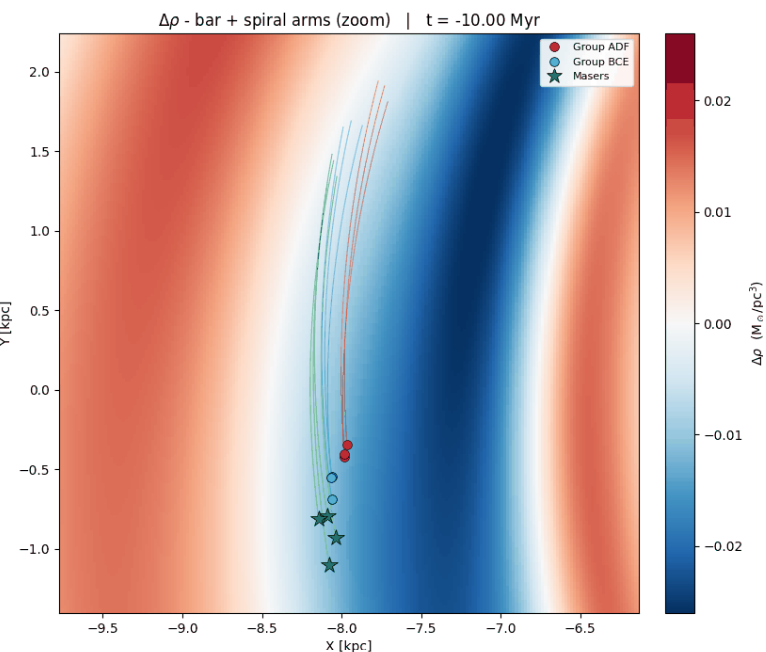
\includegraphics[height=6cm]{traj_spirale.png}
		\caption{Trajectoire des objets du Cygne selon le plan galactique depuis $-10 \ \mathrm{Myr}$, les nuages sont en vert, les groupes d'étoiles OB en rouge et bleu. Les lignes représentent la trajectoire des objets de $-10 \ \mathrm{Myr}$ à aujourd'hui. Les couleurs du fond représentent le gradient de densité, le rouge indique un milieu plus dense tandis que le bleu indique un milieu moins dense. Le potentiel gravitationnel est composé du potentiel standard avec la barre centrale galactique et l'influence des bras spiraux.}
		\label{fig:traj_spirale}
	\end{figure}
	
	\section{Conclusion}
	Ce stage a permis d'établir un tableau de données correspondant aux positions et aux vitesses de quatre nuages moléculaires ainsi que de six groupes d'étoiles massives au sein de la région du Cygne dans différents référentiels et modes de coordonnées, en utilisant les hypothèses récentes sur la vitesse et la position du Soleil. Ces données pourront être utilisés pour continuer l'étude des nuages et des amas de la région du Cygne. J'ai pu ensuite réaliser un traceback linéaire des positions des objets du Cygne à partir des vitesses calculées et retrouver leur "Time of Closest Approach" correspondant à l'évènement de formation des étoiles massives. Cela m'a permis d'identifier trois temporalités caractéristiques: l'état actuel correspondant à la collision entre les nuages existants, l'état d'il y a $4.5 \ \mathrm{Myr}$ correspondant à la collision entre les nuages des groupes B,E et C, et enfin l'état d'il y a $9.8\ \mathrm{Myr}$ correspondant à la collision des nuages des groupes F,A et D.
	En collaboration avec l'Université de Strasbourg, nous avons pu effectuer un traceback plus précis des objets du Cygne grâce à la modélisation d'un potentiel gravitationnel prenant en compte l'influence de la barre centrale et des bras spiraux. Les TCA obtenus concordent avec l'approximation linéaire et concordent aussi avec les âges stellaires de la littérature.
	Ces données et ces analyses nous ont permis de proposer un scénario de formation des étoiles massives au sein de la région du Cygne, en relevant l'importance de la propagation du bras spiral galactique dans la dynamique des nuages moléculaires. La superposition des trajectoires avec le bras Local a permis de confirmer que la région du Cygne se situe sur le bord du bras Local. Ainsi, le bras galactique serait responsable de la création de vitesses différentielles importantes entre les nuages menant à leur collision indirectes qui engendrerait la formation de groupes d'étoiles O et B.
	Ce scénario est établi uniquement sur la région du Cygne, il serait très intéressant de le confronter à l'étude d'autres régions actives comme Vega ou le Chameleon. Il serait aussi intéressant d'étudier d'autres galaxies proches où l'on peut directement distinguer les bras spiraux pour approfondir la dynamique des bras spiraux et leur influence sur la formation d'étoiles massives.
	

	\bibliographystyle{alpha}
	\nocite{*}
	\bibliography{sample}
	\textbf{Outils}
	
	Formatage LaTeX: Gemini AI / TeX Studio
	
	Code Python: Visual Studio / Github Copilot / Astropy
	
	Astronomie: Simbad / Aladin / Nasa Sky View
	
	L'ensemble du projet python est disponible sur \href{https://github.com/KyuriTaima/CygnusDynamics}{GitHub}
	
	\newpage
	
	\appendix
	\section{Données cinématiques complémentaires}
	\label{annexe:donnees_complémentaires}
		\begin{table}[H]
			\centering
			\vspace{0.2cm}
			
			\resizebox*{\textwidth}{!}{
				\begin{tabular}{l c c c c c c c c c c c c}
					\hline
					\textbf{Objet} & \textbf{RA} & \textbf{Dec} & $\mathbf{l}$ & $\mathbf{b}$ & \textbf{Distance} & $\mathbf{\mu_\alpha}$ & $\mathbf{\mu_\delta}$ & $\mathbf{\mu_l}$ & $\mathbf{\mu_b}$ & $\mathbf{V_{rad}}$ & $\mathbf{V_{LSR}}$ \\
					& ($^\circ$) & ($^\circ$) & ($^\circ$) & ($^\circ$) & ($\mathrm{pc}$) & ($\mathrm{mas/an}$) & ($\mathrm{mas/an}$) & ($\mathrm{mas/an}$) & ($\mathrm{mas/an}$) & ($\mathrm{km/s}$) & ($\mathrm{km/s}$) \\
					\hline
					
					Group A & $301.45$ & $35.68$ & $72.61$ & $2.06$ & $1894.5 \pm 10$ & -- & -- & $-6.90 \pm 0.24$ & $-1.35 \pm 0.17$ & $-12.50 \pm 2.77$ & -- \\
					Group B & $304.37$ & $41.43$ & $78.58$ & $3.31$ & $1726.3 \pm 10$ & -- & -- & $-5.47 \pm 0.34$ & $-0.59 \pm 0.27$ & $-21.00 \pm 10.80$ & -- \\
					Group C & $305.47$ & $37.87$ & $76.11$ & $0.54$ & $1713.1 \pm 10$ & -- & -- & $-6.57 \pm 0.27$ & $-1.19 \pm 0.12$ & $-19.20 \pm 2.98$ & -- \\
					Group D & $304.34$ & $37.64$ & $75.44$ & $1.19$ & $2000.1 \pm 10$ & -- & -- & $-5.55 \pm 0.16$ & $-1.34 \pm 0.14$ & $-7.00 \pm 3.88$ & -- \\
					Group E & $308.08$ & $41.30$ & $80.19$ & $0.85$ & $1674.0 \pm 10$ & -- & -- & $-4.72 \pm 0.27$ & $-0.96 \pm 0.25$ & $-12.35 \pm 2.06$ & -- \\
					Group F & $302.95$ & $36.58$ & $74.04$ & $1.44$ & $1985.2 \pm 10$ & -- & -- & $-6.11 \pm 0.30$ & $-1.33 \pm 0.10$ & $-13.48 \pm 5.06$ & -- \\
					W75N & $309.65$ & $42.63$ & $81.87$ & $0.78$ & $1300 \pm 70$ & $-4.50 \pm 0.01$ & $-0.96 \pm 0.01$ & -- & -- & -- & $9.00$ \\
					DR21 & $309.76$ & $42.42$ & $81.75$ & $0.59$ & $1500 \pm 80$ & $-4.74 \pm 0.01$ & $-0.06 \pm 0.01$ & -- & -- & -- & $-3.00$ \\
					DR20 & $309.25$ & $41.58$ & $80.86$ & $0.38$ & $1460 \pm 90$ & $-5.84 \pm 0.01$ & $-0.29 \pm 0.01$ & -- & -- & -- & $-3.00$ \\
					IRAS20290 & $307.71$ & $41.04$ & $79.74$ & $0.99$ & $1360 \pm 120$ & $-5.02 \pm 0.02$ & $-0.15 \pm 0.02$ & -- & -- & -- & $-1.40$ \\
					\hline
				\end{tabular}
			}
			\caption{Données astrométriques et cinématiques brutes de la littérature (Quintana et al. 2021 ; Rygl et al. 2012) utilisées en entrée.}
			\label{tab:annexe_donnees_entree}
		\end{table}
		\begin{table}[H]
			\centering
			\vspace{0.2cm}
			
			\resizebox{0.9\textwidth}{!}{
				\begin{tabular}{l c c c c}
					\hline
					\textbf{Objet} & $\mathbf{X_{helio}}$ & $\mathbf{Y_{helio}}$ & $\mathbf{Z_{helio}}$ & $\mathbf{\beta}$ \\
					& ($\mathrm{pc}$) & ($\mathrm{pc}$) & ($\mathrm{pc}$) & ($\mathrm{rad}$) \\
					\hline
					Group A & $566 \pm 1$ & $1807 \pm 4$ & $68.1 \pm 0.1$ & $0.23$ \\
					Group B & $341 \pm 1$ & $1689 \pm 7$ & $99.7 \pm 0.4$ & $0.21$ \\
					Group C & $411 \pm 2$ & $1660 \pm 10$ & $16.15 \pm 0.09$ & $0.21$ \\
					Group D & $503 \pm 2$ & $1940 \pm 10$ & $41.5 \pm 0.2$ & $0.25$ \\
					Group E & $285 \pm 2$ & $1650 \pm 10$ & $24.8 \pm 0.2$ & $0.21$ \\
					Group F & $546 \pm 3$ & $1910 \pm 10$ & $49.9 \pm 0.3$ & $0.25$ \\
					W75N & $180 \pm 10$ & $1290 \pm 70$ & $17.7 \pm 0.9$ & $0.16$ \\
					DR21 & $215 \pm 11$ & $1480 \pm 80$ & $15.4 \pm 0.8$ & $0.18$ \\
					DR20 & $232 \pm 14$ & $1440 \pm 90$ & $9.7 \pm 0.6$ & $0.18$ \\
					IRAS20290 & $240 \pm 20$ & $1340 \pm 120$ & $24 \pm 2$ & $0.17$ \\
					\hline
				\end{tabular}
			}
			\caption{Coordonnées cartésiennes héliocentriques et angle d'azimut ($\beta$) calculés pour les objets de la région du Cygne. Les incertitudes sont propagées à partir des données de distance et de position de la littérature (Quintana et al. 2021 ; Rygl et al. 2012).}
			\label{tab:annexe_positions}
		\end{table}
		
		\begin{table}[H]
			\centering
			\vspace{0.2cm}
			
			\resizebox*{\textwidth}{!}{
				\begin{tabular}{l c c c c c c c}
					\hline
					\textbf{Objet} & $\mathbf{U_{obs}}$ & $\mathbf{V_{obs}}$ & $\mathbf{W_{obs}}$ & $\mathbf{U_{lsr}}$ & $\mathbf{V_{lsr}}$ & $\mathbf{W_{lsr}}$ & $\mathbf{V_{lsr,abs}}$ \\
					& \multicolumn{3}{c}{($\mathrm{km/s}$)} & \multicolumn{3}{c}{($\mathrm{km/s}$)} & ($\mathrm{km/s}$) \\
					\hline
					Group A & $56 \pm 2$ & $-30 \pm 3$ & $-13 \pm 2$ & $65 \pm 2$ & $-21 \pm 3$ & $-5 \pm 2$ & $213 \pm 4$ \\
					Group B & $40 \pm 3$ & $-29 \pm 11$ & $-6 \pm 2$ & $49 \pm 3$ & $-20 \pm 11$ & $2 \pm 2$ & $214 \pm 11$ \\
					Group C & $47 \pm 2$ & $-31 \pm 3$ & $-10 \pm 1$ & $56 \pm 2$ & $-23 \pm 3$ & $-2 \pm 1$ & $212 \pm 4$ \\
					Group D & $49 \pm 2$ & $-20 \pm 4$ & $-13 \pm 1$ & $58 \pm 2$ & $-11 \pm 4$ & $-5 \pm 1$ & $224 \pm 5$ \\
					Group E & $35 \pm 2$ & $-18 \pm 2$ & $-8 \pm 2$ & $44 \pm 2$ & $-10 \pm 2$ & $0 \pm 2$ & $225 \pm 4$ \\
					Group F & $52 \pm 3$ & $-28 \pm 5$ & $-13 \pm 1$ & $61 \pm 3$ & $-20 \pm 5$ & $-5 \pm 1$ & $215 \pm 6$ \\
					W75N & $26.4 \pm 1.5$ & $-11.5 \pm 0.2$ & $-6.0 \pm 0.3$ & $35.5 \pm 1.5$ & $-2.8 \pm 0.3$ & $1.9 \pm 0.4$ & $232 \pm 3$ \\
					DR21 & $31 \pm 2$ & $-24.3 \pm 0.3$ & $-0.63 \pm 0.07$ & $40 \pm 2$ & $-15.7 \pm 0.4$ & $7.27 \pm 0.15$ & $219 \pm 3$ \\
					DR20 & $37 \pm 2$ & $-26.0 \pm 0.4$ & $-2.14 \pm 0.14$ & $46 \pm 2$ & $-17.3 \pm 0.5$ & $5.8 \pm 0.2$ & $218 \pm 3$ \\
					IRAS20290 & $29 \pm 3$ & $-23.9 \pm 0.5$ & $-1.29 \pm 0.15$ & $38 \pm 3$ & $-15.2 \pm 0.6$ & $6.6 \pm 0.2$ & $220 \pm 3$ \\
					\hline
				\end{tabular}
			}
			\caption{Tableau récapitulatif des composantes de vitesse dans différents référentiels: référentiel observé, LSR local, puis LSR absolu incluant la rotation galactique.}
			\label{tab:annexe_vitesses_intermediaires}
		\end{table}
		\begin{table}[H]
			\centering
			\vspace{0.2cm}
			
			\resizebox{0.9\textwidth}{!}{
				\begin{tabular}{l c c c}
					\hline
					\textbf{Objet} & \textbf{Masse Stellaire Totale} & $\mathbf{\nabla v_l}$ & $\mathbf{\nabla v_b}$ \\
					& ($\mathrm{M_\odot}$) & ($\mathrm{km\cdot s^{-1}\cdot pc^{-1}}$) & ($\mathrm{km\cdot s^{-1}\cdot pc^{-1}}$) \\
					\hline
					
					Group A & $2344^{+275}_{-252}$ & $0.07 \pm 0.02$ & $0.09 \pm 0.01$ \\
					Group B & $1978^{+245}_{-224}$ & $0.11 \pm 0.01$ & $-0.01 \pm 0.01$ \\
					Group C & $2165^{+245}_{-224}$ & $0.10 \pm 0.01$ & $0.03 \pm 0.01$ \\
					Group D & $1569^{+215}_{-192}$ & $0.05 \pm 0.01$ & $0.02 \pm 0.01$ \\
					Group E & $4198^{+354}_{-319}$ & $0.12 \pm 0.01$ & $0.04 \pm 0.01$ \\
					Group F & $2955^{+349}_{-269}$ & $0.09 \pm 0.01$ & $0.02 \pm 0.01$ \\
					W75N & -- & -- & -- \\
					DR21 & -- & -- & -- \\
					DR20 & -- & -- & -- \\
					IRAS20290 & -- & -- & -- \\
					\hline
				\end{tabular}
			}
			\caption{Propriétés physiques et cinématiques internes des amas stellaires. L'ensemble de ces données proviennent de Quintana et al. 2021. Ces valeurs ne sont pas disponibles pour les nuages moléculaires}
			\label{tab:annexe_masses_gradients}
		\end{table}
		
	\section{Méthode de calcul des incertitudes}
	\label{annexe:methode_incertitudes}
	Pour les transformations linéaires, je propage les incertitudes en utilisant la formule de propagation des incertitudes de Taylor \cite{taylor1997} du premier ordre:
	$$\Delta f(u_1,...,u_n) = \sqrt{\sum_{i=1}^{n} \left(\frac{\partial f}{\partial u_i} \right)^2 (\Delta u_i)^2}$$
	
	Pour les autres, j'effectue un échantillonnage de Monte-Carlo avec un tirage de 10 000 points.
	\subsection*{Vitesse radiale}
	La projection de la vitesse du soleil dans le standard LSR dépend des incertitudes sur les longitudes et latitudes galactiques qui sont négligeables par rapport aux incertitudes sur la vitesse LSR des objets observés: 
	$$V_{RV} \ = \ v_{lsr} \ - \ v_{sun,old,proj}$$
	
	Donc: $\Delta V_{RV} \ = \ \Delta v_{lsr}$
	
	\subsection*{Vitesses héliocentriques}
	Les incertitudes sur les composantes héliocentriques $U_{helio}$, $V_{helio}$, $W_{helio}$ sont dérivées des incertitudes sur les mouvements propres et les composantes de vitesse du Soleil. La transformation est non linéaire donc elles sont propagées par méthode de Monte-Carlo.
	
	\subsection*{Vitesses LSR}
	\begin{equation}
		U_{lsr} = U_{obs} + U_{\odot} \quad ; \quad V_{lsr} = V_{obs} + V_{\odot} \quad ; \quad W_{lsr} = W_{obs} + W_{\odot}
	\end{equation}
	C'est une addition simple donc je peux obtenir l'incertitude par la formule de propagation des incertitudes:
	
	\begin{align}
		\Delta U_{lsr} &= \sqrt{(\Delta U_{obs})^2 + (\Delta U_{\odot})^2} \\
		\Delta V_{lsr} &= \sqrt{(\Delta V_{obs})^2 + (\Delta V_{\odot})^2} \\
		\Delta W_{lsr} &= \sqrt{(\Delta W_{obs})^2 + (\Delta W_{\odot})^2}
	\end{align}
	
	Pour la vitesse LSR corrigée de la vitesse de rotation moyenne de la galaxie: 
	
	$$V_{lsr,abs} = V_{lsr} + \Theta_0$$
	
	Donc $$\Delta V_{lsr,abs} = \sqrt{(\Delta V_{lsr})^2 + (\Delta \Theta_0)^2}$$
	
	Pour la vitesse lsr sur la ligne de visée $v_{lsr}$, l'incertitude est observationnelle pour les nuages moléculaires mais elle est calculée pour les amas d'étoiles.
	$$v_{lsr} \ = \ V_{RV} + v_{sun,proj,old} \ \implies \ \Delta v_{lsr} \ = \ \Delta V_{RV}$$  
	
	\subsection*{Composantes U, V et W dans le référentiel galactocentrique particulier}
	Le référentiel galactocentrique particulier est le référentiel LSR déplacé au niveau de l'objet observé. L'angle $\beta$ est déterminé à partir des angles $l$ et $b$ qui ont des incertitudes très faibles. Donc les incertitudes sur $\beta$ peuvent être négligées par rapport aux incertitudes sur les vitesses:
	\begin{align}
		U_{pec} &= U_{lsr,abs} \cos(\beta) - V_{lsr,abs} \sin(\beta) \\
		V_{pec} &= U_{lsr,abs} \sin(\beta) + V_{lsr,abs} \cos(\beta) - \Theta_0 \\
		W_{pec} &= W_{lsr,abs}
	\end{align}
	
	\begin{align}
		\Delta U_{pec} &= \sqrt{\cos^2(\beta) \Delta U_{lsr,abs}^2 + \sin^2(\beta) \Delta V_{lsr,abs}^2} \\
		\Delta V_{pec} &= \sqrt{\sin^2(\beta) \Delta U_{lsr,abs}^2 + \cos^2(\beta) \Delta V_{lsr,abs}^2 + \Delta\Theta_0^2} \\
		\Delta W_{pec} &= \Delta W_{lsr,abs}
	\end{align}
	
	\subsection*{Vitesses selon les coordonnées galactiques}
	Les vitesses selon les coordonnées galactiques $v_l$ et $v_b$ sont calculées analytiquement, donc leut incertitude est propagée selon la formule de propagation des incertitudes.
	\begin{align}
		v_l &= -U_{pec} \sin(l) + V_{pec} \cos(l) \\
		\Delta v_l &= \sqrt{\sin^2(l) \Delta U_{pec}^2 + \cos^2(l) \Delta V_{pec}^2} \\[1.5em]
		v_b &= -U_{pec} \cos(l) \sin(b) - V_{pec} \sin(l) \sin(b) + W_{pec} \cos(b) \\
		\Delta v_b &= \sqrt{\cos^2(l)\sin^2(b) \Delta U_{pec}^2 + \sin^2(l)\sin^2(b) \Delta V_{pec}^2 + \cos^2(b) \Delta W_{pec}^2} \\[1.5em]
		v_{lb} &= \sqrt{v_l^2 + v_b^2} \\
		\Delta v_{lb} &= \sqrt{\frac{v_l^2}{v_l^2 + v_b^2} \Delta v_l^2 + \frac{v_b^2}{v_l^2 + v_b^2} \Delta v_b^2}
	\end{align}
	
	\section{Graphiques complémentaires}
	\label{appendix:complementary_graphs}
	Je trace les mouvements propres selon la longitude galactique $\mu_b$ en fonction de la longitude galactique en figure \ref{fig:proper_motion_galactic_longitude}. Quintana et al. avaient interprété la linéarité de $\mu_l$ en fonction de $l$ comme un signe d'appartenance à un même super-groupe. On retrouve bien les super-groupes d'amas d'étoiles et on remarque une linéarité entre W75N, DR21 et DR20, ce qui appuie l'hypothèse de leur appartenance à un même groupe cinématique cohérent. Cependant, IRAS20290+4052 s'intègre mal à ce super-groupe de nuages moléculaires selon le graphique.
	
	\begin{figure}[H]
		\centering
		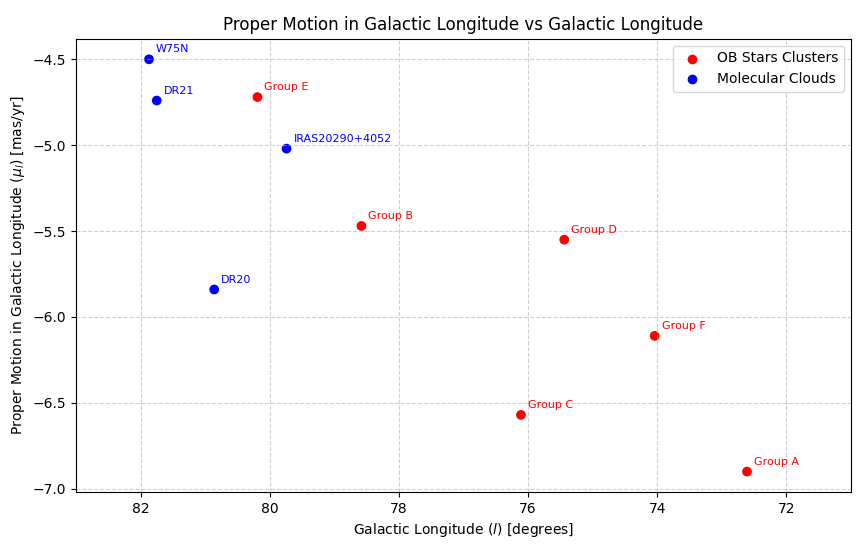
\includegraphics[height=10cm]{mu_l as a fct of l.png}
		\caption{Mouvement propre selon la longitude galactique $\mu_l$ en fonction de la longitude galactique $l$, les nuages moléculaires sont en bleus et les amas d'étoiles OB en rouge}
		\label{fig:proper_motion_galactic_longitude}
	\end{figure}
	
	Je trace aussi $\mu_l$ en fonction de $\mu_b$ figure \ref{fig:proper_motions}, mais aucun regroupement particulier n'en ressort.
	
	\begin{figure}[H]
		\centering
		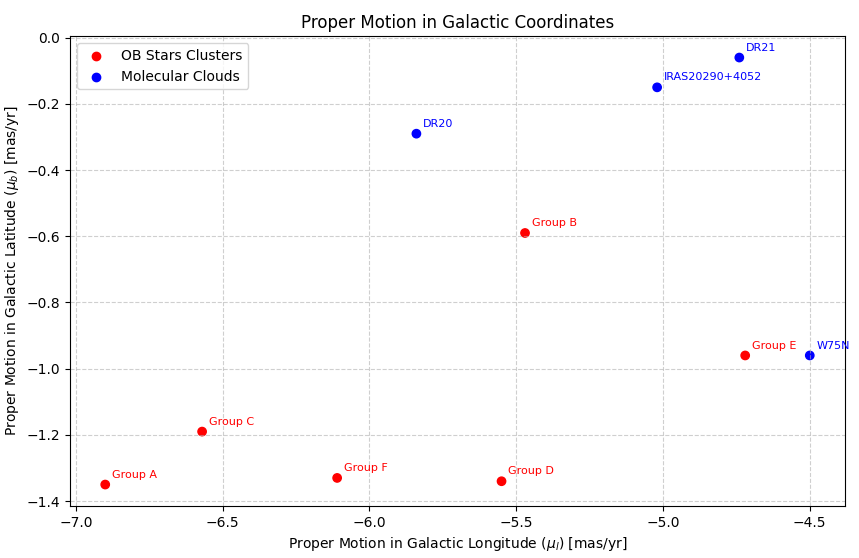
\includegraphics[height=8cm]{mu_b as a fct of mu_l.png}
		\caption{Mouvement propre selon la latitude galactique $\mu_b$ en fonction du mouvement propre selon la longitude galactique $\mu_l$, les nuages moléculaires sont en bleus et les amas d'étoiles OB en rouge}
		\label{fig:proper_motions}
	\end{figure}
	
	\begin{figure}[H]
		\centering
		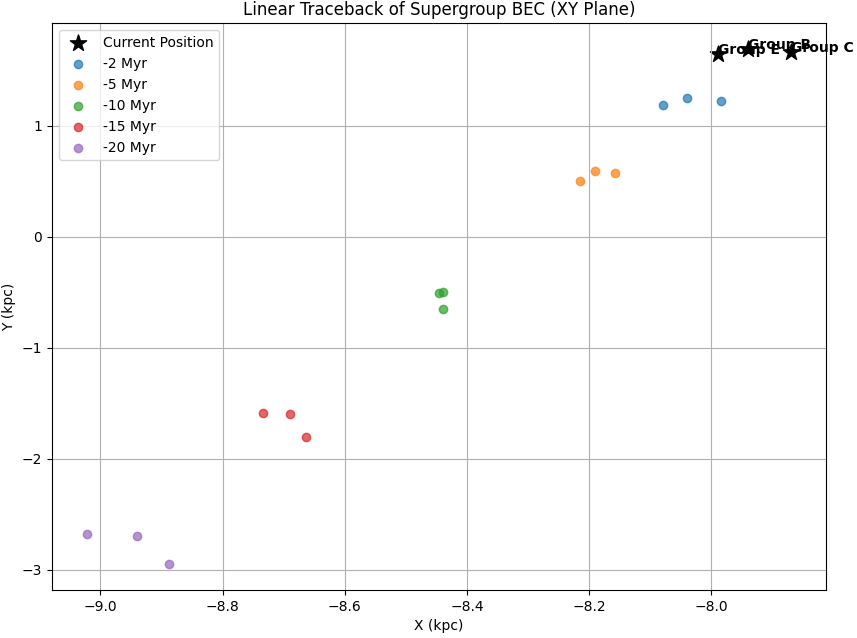
\includegraphics[height=10cm]{linear_traceback_BEC_XY.png}
		\caption{Traceback linéaire des amas d'étoiles du super-groupe BEC selon le plan galactique. L'axe des abscisses représente la distance au centre galactique, et l'axe des ordonnées représente la tangente à la trajectoire de rotation moyenne de la galaxie au niveau du Cygne.}
		\label{fig:linear_traceback_BEC_XY}
	\end{figure}
	
	\begin{figure}[H]
		\centering
		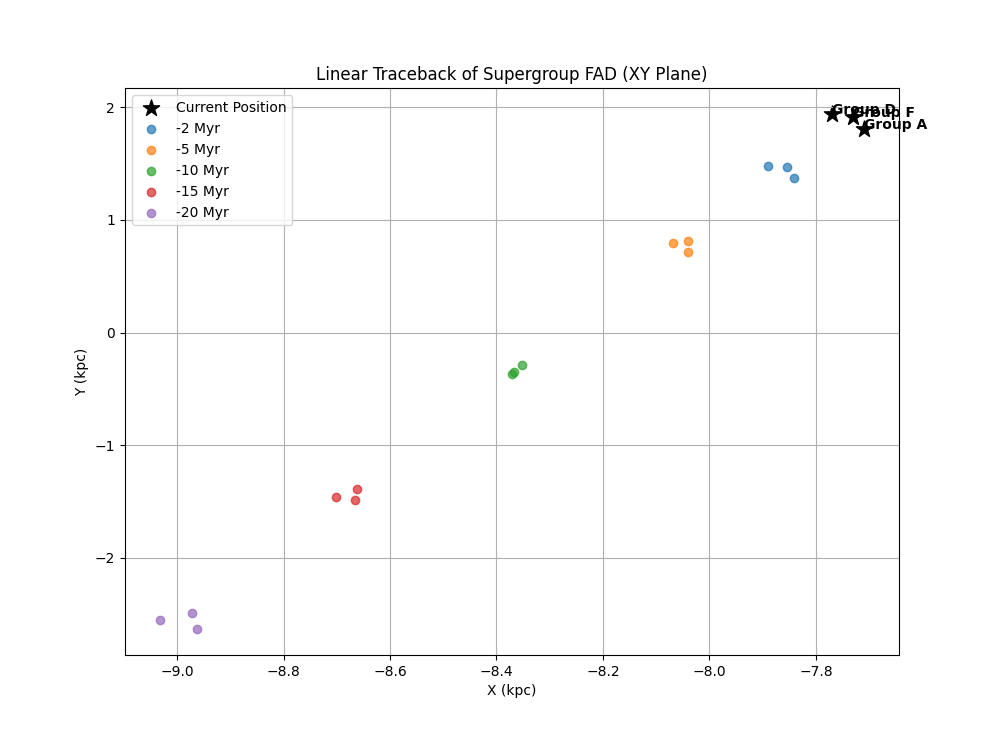
\includegraphics[height=10cm]{linear_traceback_FAD_XY.png}
		\caption{Traceback linéaire des amas d'étoiles du super-groupe FAD selon le plan galactique. L'axe des abscisses représente la distance au centre galactique, et l'axe des ordonnées représente la tangente à la trajectoire de rotation moyenne de la galaxie au niveau du Cygne.}
		\label{fig:linear_traceback_FAD_XY}
	\end{figure}
	
	\begin{figure}[H]
		\centering
		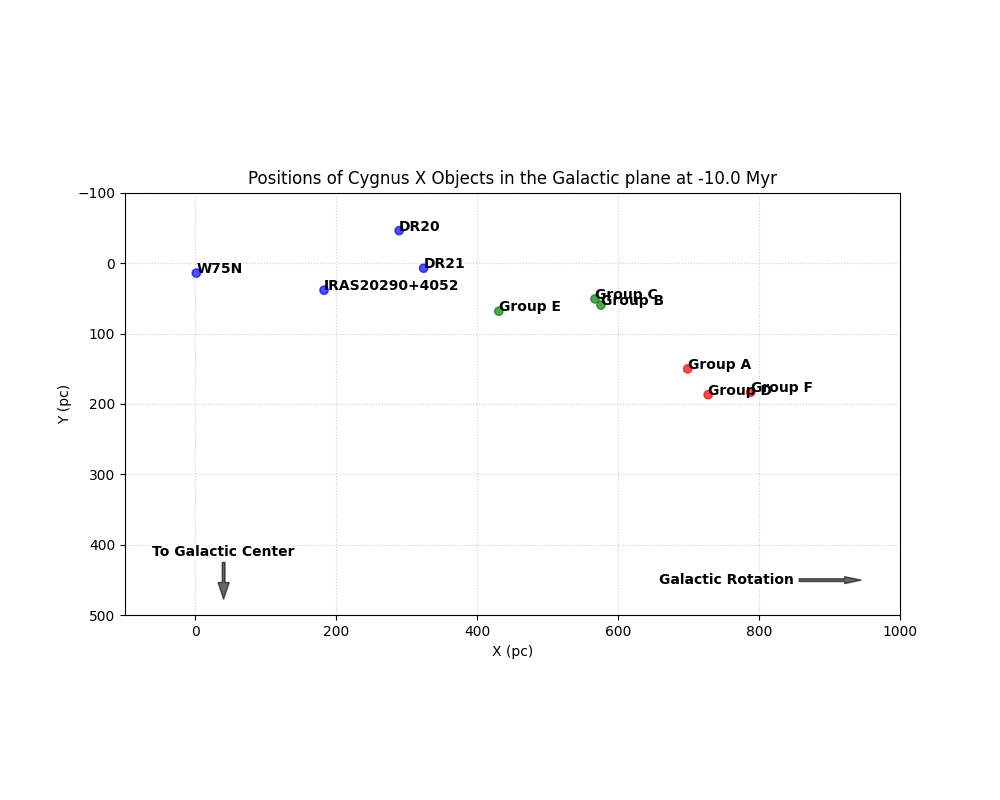
\includegraphics[width=0.8\textwidth, height=8cm, keepaspectratio]{traceback_gal_plane_10.png}
		
		\vspace{0.4cm}
		
		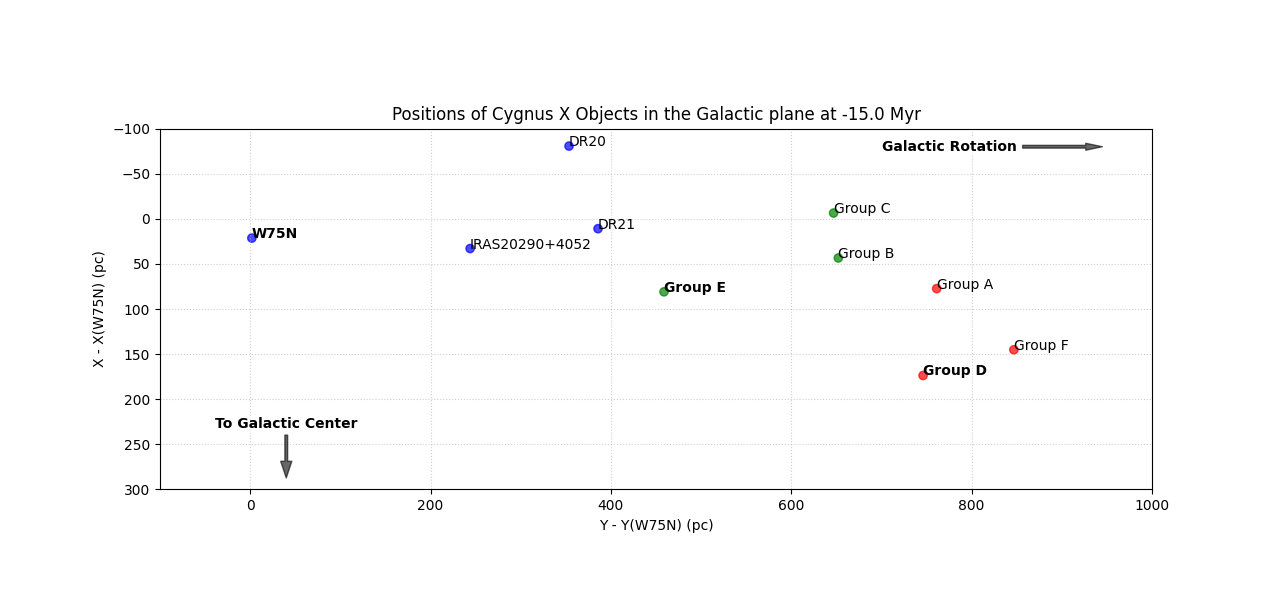
\includegraphics[width=0.8\textwidth, height=8cm, keepaspectratio]{traceback_gal_plane_15.png} 
		\caption{ le plan galactique des objets du Cygne à $-10$ et $-15 \ \mathrm{Myr}$. L'origine est la position actuelle du nuage W75N.}
		\label{fig:traceback_complémentaires}
	\end{figure}
	
	\begin{figure}[H]
		\centering
		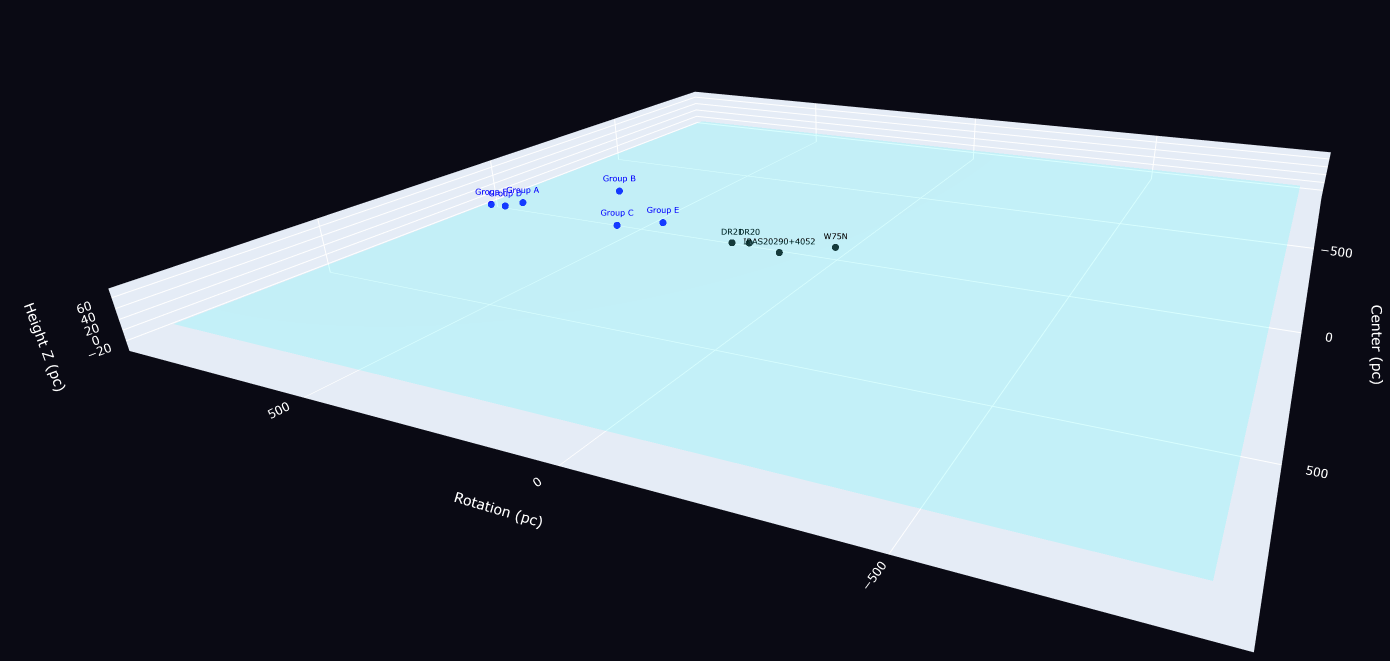
\includegraphics[width=0.8\textwidth, height=10cm, keepaspectratio]{traceback_3D_4,5.png}
		
		\vspace{0.4cm}
		
		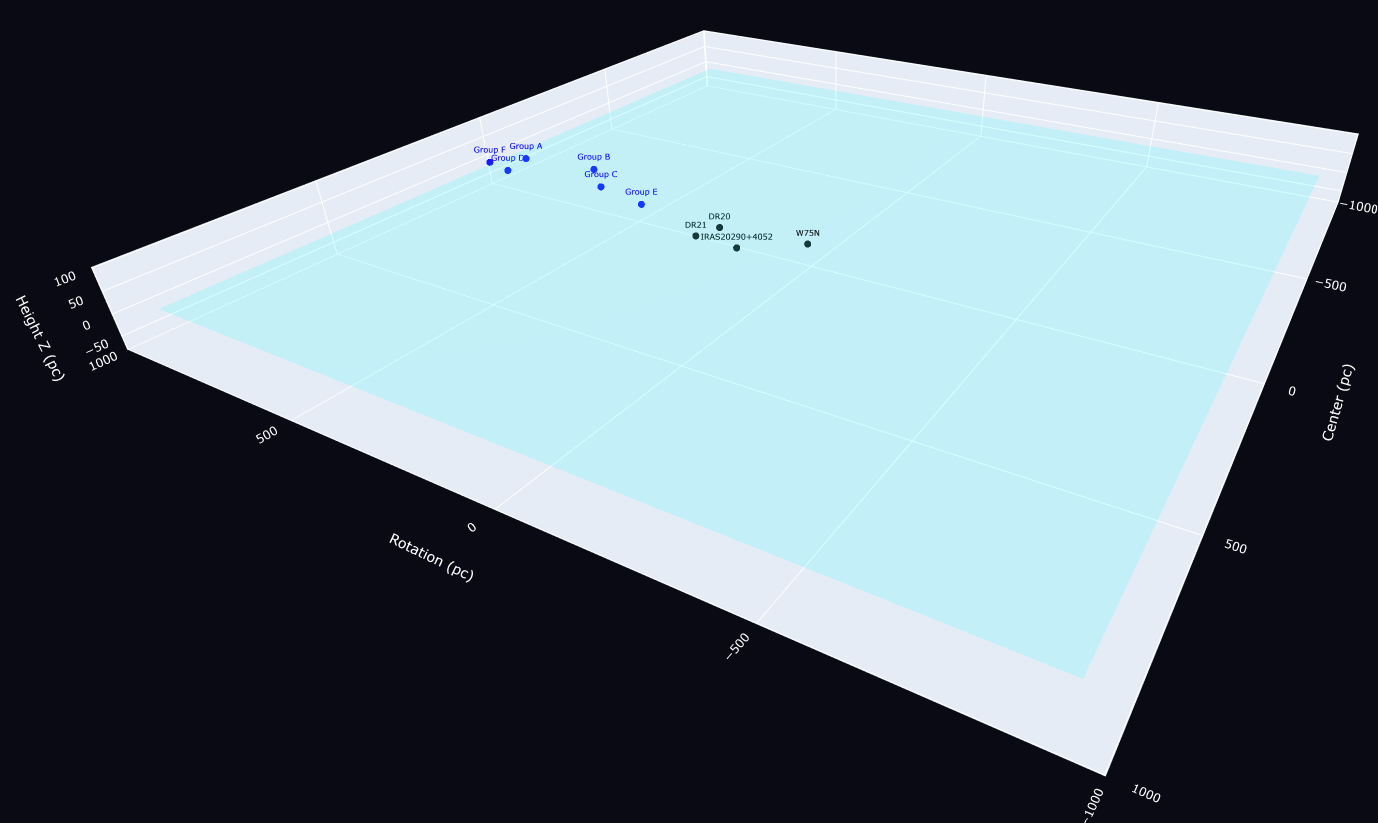
\includegraphics[width=0.8\textwidth, height=10cm, keepaspectratio]{traceback_3D_9,8.png} 
		\caption{Traceback linéaire modélisé en 3D des objets du Cygne à $-4.5$ et $-9.8 \ \mathrm{Myr}$. L'origine est la position actuelle du nuage W75N.}
		\label{fig:traceback_complémentaires_3D}
	\end{figure}
	
	\begin{figure}[H]
		\centering
		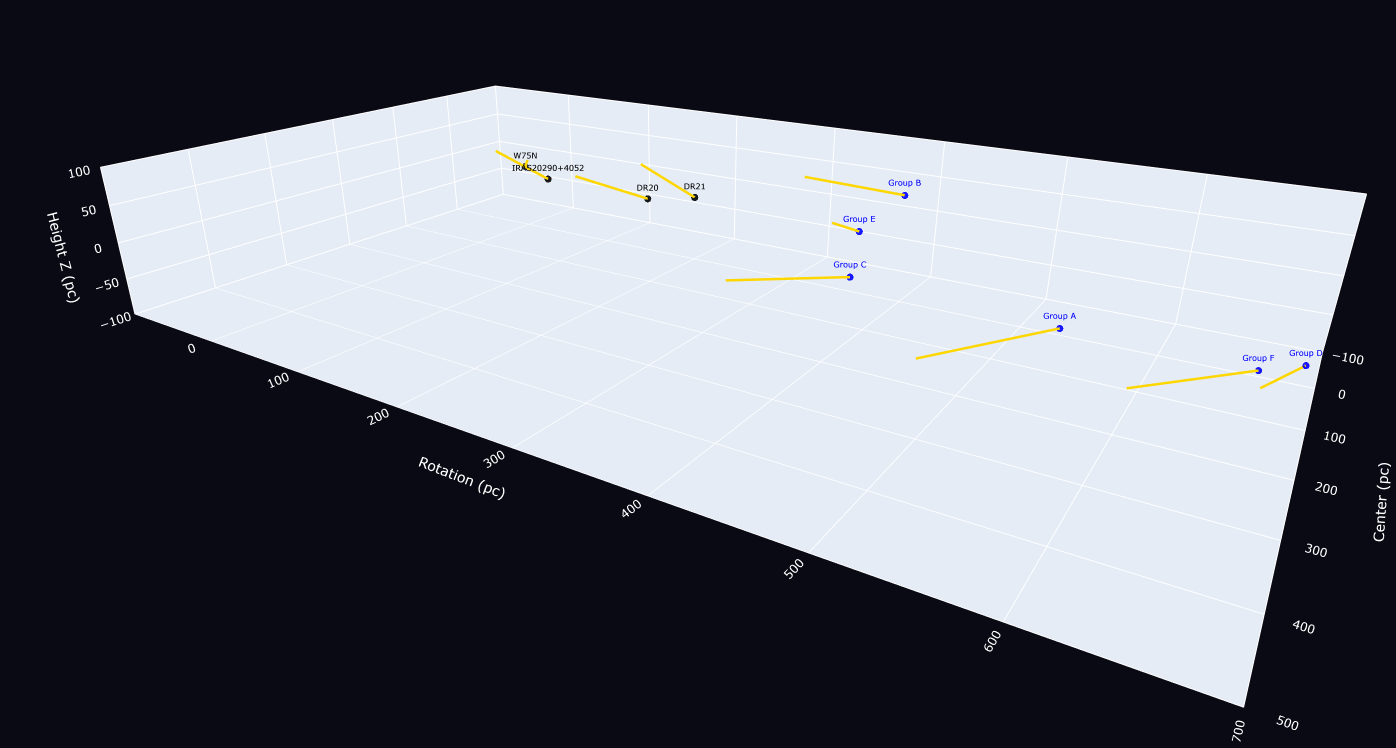
\includegraphics[height=8cm]{3D_view_1.png}
		\caption{Visualisation des objets du Cygne en 3D dans le repère centré sur W75N. Les lignes jaunes représentent les vecteurs vitesses}
		\label{fig:3D_view_1}
	\end{figure}
	
	\begin{figure}[H]
		\centering
		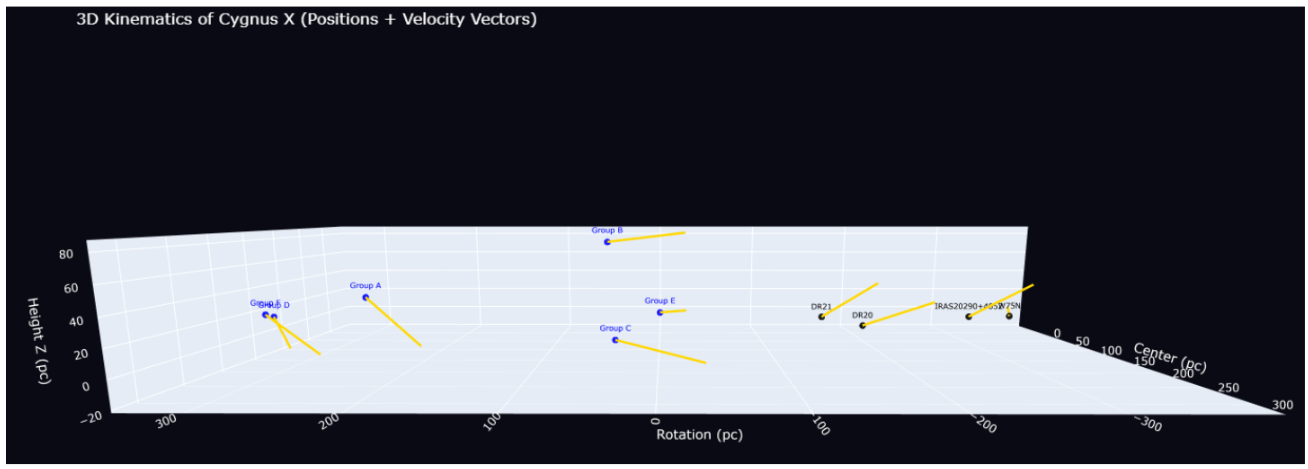
\includegraphics[height=8cm]{3D_view_2.png}
		\caption{Visualisation des objets du Cygne en 3D dans le repère centré sur W75N. Les lignes jaunes représentent les vecteurs vitesses}
		\label{fig:3D_view_2}
	\end{figure}
	
	\begin{figure}[H]
		\centering
		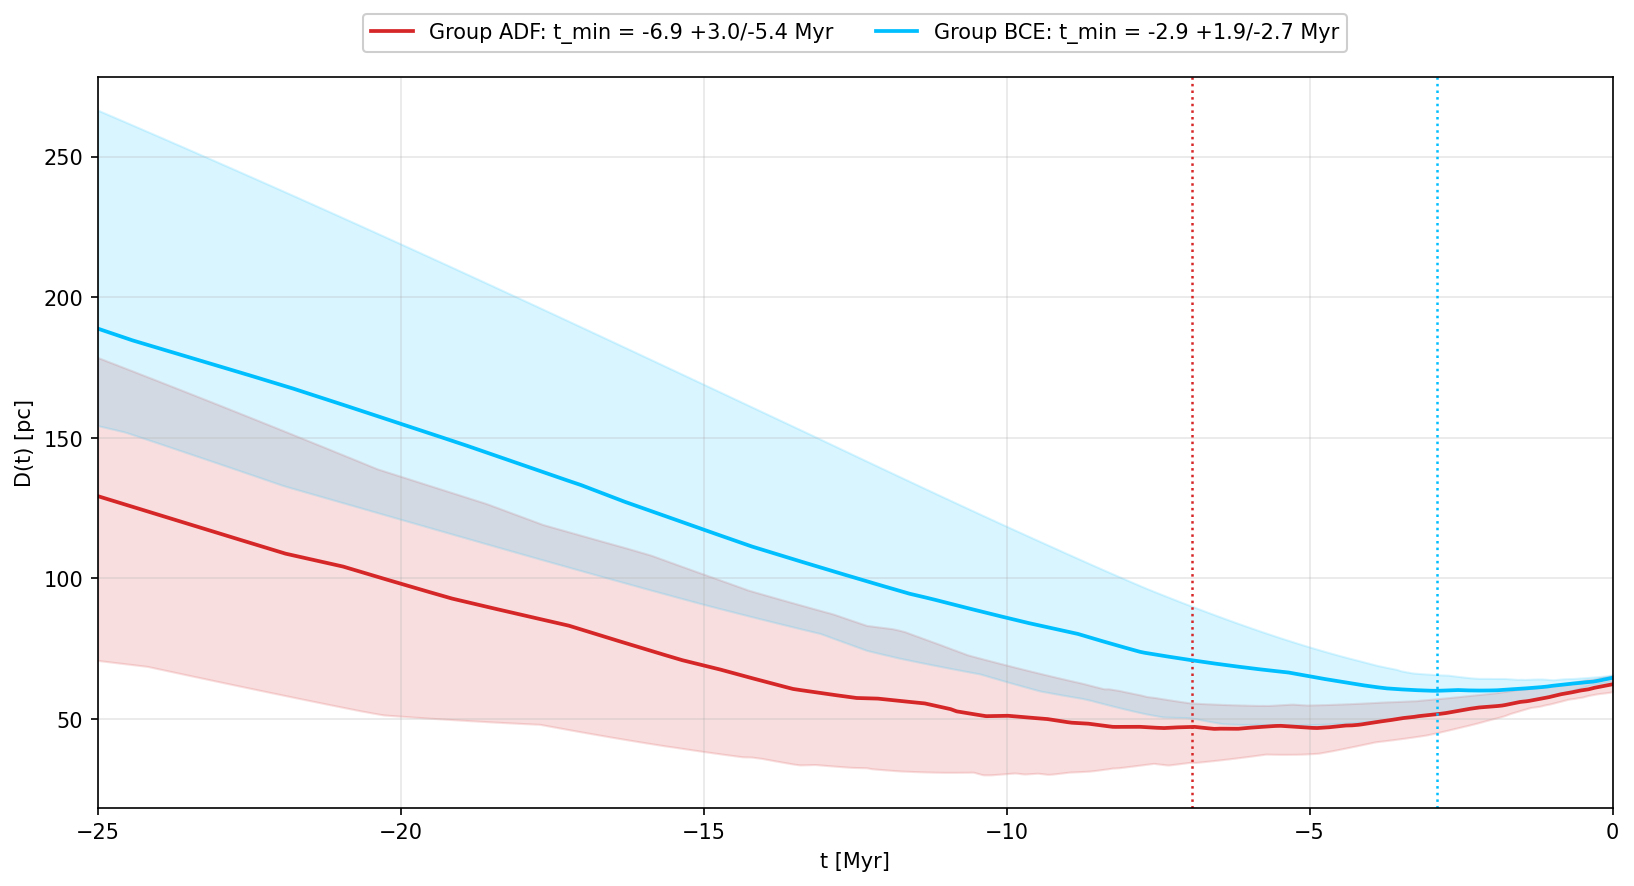
\includegraphics[height=6cm]{TCA_nonaxi.png}
		\caption{TCA obtenus avec un potentiel gravitationnel local non axi-symétrique par Y. Khalil}
		\label{fig:TCA_nonaxi}
	\end{figure}
	
	\section{Calculs de traceback linéaires}
	\label{appendix:linear_traceback}
	
	Je détermine les coordonnées $x(t)$, $y(t)$, et $z(t)$ de chaque objet à un instant $t$ dans le passé. Avec $V_x$, $V_y$ et $V_z$ les vitesses des objets selon les axes $\vec{x}$, $\vec{y}$, $\vec{z}$.
	
	\begin{align}
		x(t) \ = \ x(0) \ - \ V_xt \\
		y(t) \ = \ y(0) \ - \ V_yt \\
		z(t) \ = \ z(0) \ - \ V_zt \\
	\end{align}
	
	Et je détermine la distance euclidienne entre chaque objet d'un super-amas à l'instant t:
	$$d \ = \ \sqrt{(x_1(t) \ - \ x_2(t))^2 \ + \ (y_1(t) \ - \ y_2(t))^2 \ + \ (z_1(t) \ - \ z_2(t))^2}$$
	
	Puis je prend la moyenne des trois distances à l'instant $t$, l'instant $t$ correspondant à la valeur minimale est le "Time of Closest Approach".
	
	\newpage
	
	\begin{abstract}
		\begin{center}
			\textbf{\Large Cinématique des étoiles jeunes et du gaz moléculaire dans le complexe Cygnus-X} \\
			\vspace{0.2cm}
			\textit{Université de Bordeaux / Laboratoire d'Astrophysique de Bordeaux} \\
			\vspace{0.5cm}
		\end{center}
		
		\noindent Directeur de stage : Sylvain Bontemps
		
		\vspace{1cm}
		
		\textbf{Français} \\
		
		La cinématique des étoiles massives de type OB reste mal corrélée à celle des nuages moléculaires environnants. Je me suis intéressé à la région du Cygne ($1,5 \ \mathrm{kpc}$).J'ai d'abord généré une table de données cinématiques multi-référentiels, basée sur les paramètres solaires les plus récents. J'ai ensuite modélisé ces objets en trois dimensions, puis simulé leur trajectoire par un retour en arrière cinématique (\textit{traceback}). L'analyse a mis en évidence deux super-amas distincts, composés de trois groupes chacun, dont les temps de formation dynamiques ont été estimés à $4 \ \mathrm{Myr}$ et $8 \ \mathrm{Myr}$. Les trajectoires ont révélé qu'un retard cinématique d'une partie du gaz a provoqué un scénario de collision indirecte, répété à trois époques distinctes. Enfin, en superposant les trajectoires des objets avec la position des bras galactique, nous avons constaté que la formation d'étoiles massives a lieu sur les bords du bras Local, et que les bras galactiques jouent un rôle dans la dynamique des nuages moléculaires engendrant des collisions, et ultimement la formation de groupes d'étoiles massives.
		
		\textbf{Mots clés:} Formation d'étoiles OB - Cygnus X - Potentiel gravitationnel - Cinématique et dynamique - Bras galactique
		
		\vspace{1.5cm}
		
		\textbf{English} \\
		
		The kinematics of massive OB-type stars remain poorly correlated with those of the surrounding molecular clouds. I focused on the Cygnus region ($1.5 \ \mathrm{kpc}$). I first generated a multi-frame kinematic data table based on the most recent solar parameters. I then modeled these objects in three dimensions and simulated their trajectories using a kinematic traceback. The analysis revealed two distinct superclusters, each composed of three groups, whose dynamic formation times were estimated at $4 \ \mathrm{Myr}$ and $8 \ \mathrm{Myr}$. The trajectories showed that a kinematic lag in a portion of the gas led to an indirect collision scenario, which recurred at three distinct epochs. Finally, by superimposing the object trajectories onto the positions of the galactic arms, we found that massive star formation occurs at the edges of the Local Arm, and that the galactic arms play a role in the dynamics of molecular clouds, leading to collisions and, ultimately, the formation of massive star clusters.
		
		\textbf{Keywords:} OB Star Formation - Cygnus X - Gravitational Potential - Kinematics and Dynamics - Galactic Arm		
		
	\end{abstract}
	
\end{document}
